\documentclass[12pt,a4paper]{article}

% --------------------------------------------------
% PACKAGES
% --------------------------------------------------
\usepackage[margin=1in]{geometry}
\usepackage[T1]{fontenc}
\usepackage[utf8]{inputenc}
\usepackage{lmodern}
\usepackage{setspace}
\usepackage{graphicx}
\usepackage{booktabs}
\usepackage{array}
\usepackage{longtable}
\usepackage{amsmath}
\usepackage{xurl}
\usepackage[hidelinks]{hyperref}
\usepackage{float}
\usepackage{caption}
\usepackage{enumitem}
\usepackage{placeins}
% Figures are placed exactly where they are declared using the [H] placement option.

\hypersetup{
	colorlinks=true,
	linkcolor=blue,
	urlcolor=blue,
	citecolor=blue
}
\urlstyle{same}
\onehalfspacing
\setlength{\parindent}{0pt}
\setlength{\parskip}{6pt}

% --------------------------------------------------
% DOCUMENT START AND CUSTOM COVER PAGE
% --------------------------------------------------
\begin{document}
	
	% The titlepage environment creates a dedicated cover page.
	% Keep zw.png in the same Overleaf project folder as this .tex file.
	\begin{titlepage}
		\centering
		\thispagestyle{empty}
		\vspace*{0.8cm}
		
		% Zimbabwean flag appears first, above the title.
		
\includegraphics[width=0.22\textwidth]{zw.png}\par
		\vspace{1.4cm}
		
		{\Large\bfseries Zimbabwe Weather Intelligence\par}
		\vspace{0.6cm}
		
		{\large An End-to-End Machine Learning System for\\[0.25cm]
			One-Hour-Ahead Temperature Prediction Across Four Zimbabwean Cities\par}
		
		\vspace{1.8cm}
		
		{\large Rosemary Mtape\par}
		\vspace{0.3cm}
		{\normalsize MacroEdTech -- Team GenAI Research 2026\par}
		
		\vfill
		{\large October 2026\par}
		\vspace*{1cm}
	\end{titlepage}
	
	% --------------------------------------------------
	% ABSTRACT: ALWAYS STARTS ON A NEW PAGE AFTER THE COVER
	% --------------------------------------------------
	\clearpage
	\begin{abstract}
		Accurate short-term temperature prediction can support weather
		monitoring, environmental planning, and data-informed decision-making.
		This study presents Zimbabwe Weather Intelligence, an end-to-end
		machine learning application developed to predict temperature one
		hour ahead for Harare, Bulawayo, Mutare, and Gweru, Zimbabwe. The
		consolidated dataset contains 385,728 hourly records covering
		1 January 2015 to 31 December 2025.
		
		Six approaches were evaluated: a persistence baseline, Linear
		Regression, Random Forest, Extreme Gradient Boosting (XGBoost), a
		baseline Long Short-Term Memory (LSTM) model, and an improved LSTM
		configuration. The chronological evaluation used data through 2022
		for training, 2023--2024 for validation, and 2025 for testing. Among
		the evaluated models, XGBoost achieved the lowest reported test-set
		mean absolute error (MAE) of 0.3448$^\circ$C and root mean squared
		error (RMSE) of 0.5210$^\circ$C, with an $R^2$ of 0.9882. The selected
		model was integrated into a FastAPI prediction service and a Streamlit
		dashboard, deployed separately using Render and Streamlit Community
		Cloud.
		
		Seven automated API tests passed in the development environment.
		The deployed API and dashboard were also checked using the available
		health, documentation, and prediction workflows. The results
		demonstrate the feasibility of connecting historical weather data,
		machine learning, an API, and an interactive web interface. The
		reported performance applies to the specified test dataset and does
		not establish equivalent accuracy for future periods, extreme
		weather, or locations outside the study area. The dashboard uses
		user-supplied weather inputs and is not an independent live-weather
		forecasting service.
	\end{abstract}
	
	\textbf{Keywords:} weather prediction, temperature prediction,
	machine learning, XGBoost, Random Forest, LSTM, FastAPI, Streamlit,
	Zimbabwe.
	\clearpage
	\tableofcontents
	\newpage
	
	% --------------------------------------------------
	% 1. INTRODUCTION
	% --------------------------------------------------
	\section{Introduction}
	
	Weather conditions influence agriculture, water management,
	transportation, energy use, public health, and environmental
	planning. Short-term weather information can help individuals and
	organisations make better-informed operational decisions. Temperature
	is an important meteorological variable for understanding daily
	weather patterns and near-term atmospheric conditions.
	
	Conventional weather forecasting draws on meteorological observations
	and physical models of atmospheric processes. Machine learning offers
	an additional approach by learning statistical patterns from
	historical observations and estimating future outcomes from
	available input variables. Its usefulness depends on the quality
	and representativeness of the data, the features provided to the
	model, and the validity of the evaluation procedure.
	
	Zimbabwe Weather Intelligence was developed as a practical
	investigation into one-hour-ahead temperature prediction for Harare,
	Bulawayo, Mutare, and Gweru. The project combines historical data
	acquisition, preprocessing, exploratory data analysis, feature
	engineering, model comparison, API development, automated testing,
	and web application deployment.
	
	The wider project may provide a foundation for later work involving
	satellite imagery and environmental analysis. Those satellite
	experiments are separate from the deployed temperature prediction
	pipeline described and evaluated in this report.
	
	\subsection{Problem Statement}
	
	Historical weather observations contain temporal patterns and
	relationships among meteorological variables that may support
	short-term prediction. Converting such observations into an
	accessible prediction service requires more than fitting a model:
	the data must be prepared consistently, candidate algorithms must
	be evaluated appropriately, and the selected model must be integrated
	into a usable application.
	
	This study addresses how to develop and evaluate a machine learning
	pipeline for one-hour-ahead temperature prediction in selected
	Zimbabwean cities and make its predictions accessible through a
	web application and API.
	
	\subsection{Aim}
	
	The aim is to develop, evaluate, and deploy an end-to-end machine
	learning system for one-hour-ahead temperature prediction using
	historical hourly weather data from four cities in Zimbabwe.
	
	\subsection{Objectives}
	
	The objectives are to:
	\begin{enumerate}[leftmargin=*]
		\item Obtain and prepare historical hourly weather observations
		for four Zimbabwean cities.
		\item Examine the data for missing values, duplicate records,
		temporal patterns, and relationships among weather variables.
		\item Engineer temporal and historical features suitable for
		short-term temperature prediction.
		\item Develop and compare statistical, ensemble machine learning,
		and deep learning models using a chronological evaluation strategy.
		\item Select a model using test metrics and examine its feature
		importance.
		\item Develop a FastAPI prediction service and a Streamlit
		dashboard around the selected model.
		\item Test core API behaviour and deploy the application for
		public access.
	\end{enumerate}
	
	\subsection{Research Questions}
	
	The study addresses the following questions:
	\begin{enumerate}[leftmargin=*]
		\item How effectively can historical hourly weather variables
		support one-hour-ahead temperature prediction across the four
		selected cities?
		\item How do persistence, Linear Regression, Random Forest,
		XGBoost, and LSTM models compare on the evaluated test period?
		\item Which features are most influential in the selected
		XGBoost model?
		\item How can the selected model be integrated into an accessible
		and testable web application?
	\end{enumerate}
	
	\subsection{Scope}
	
	The study covers Harare, Bulawayo, Mutare, and Gweru, using hourly
	historical observations from 2015 through 2025. The prediction target
	is temperature one hour ahead. XGBoost is the model deployed in the
	application; the LSTM models are experimental alternatives.
	
	The dashboard accepts user-supplied weather values and requests a
	prediction from the API. It does not independently retrieve current
	weather observations and is not an official meteorological forecast
	or warning service.
	
	% --------------------------------------------------
	% 2. RELATED WORK
	% --------------------------------------------------
	\section{Related Work}
	
	\subsection{Machine Learning for Weather Prediction}
	
	Machine learning methods estimate relationships between input
	variables and prediction targets from historical observations.
	Their usefulness depends on data quality, feature design, evaluation
	strategy, and the similarity between training and prediction
	conditions. Regression models offer a useful baseline, ensemble
	methods can represent nonlinear relationships, and sequence models
	can learn patterns across ordered observations. No single algorithm
	is guaranteed to perform best for every location, variable, or
	forecasting horizon; empirical comparison is therefore necessary.
	
	\subsection{Linear Regression}
	
	Linear Regression estimates a continuous target as a weighted
	combination of input features; its performance is assessed here using
	standard regression metrics \cite{scikitlearnmetrics}. It provides a relatively simple
	baseline for assessing whether relationships in the data can be
	approximated linearly. Nonlinear relationships and feature
	interactions may not be represented adequately by a basic linear
	model.
	
	\subsection{Random Forest}
	
	Random Forest combines predictions from multiple decision trees
	and introduces randomness during tree construction. Breiman (2001)\cite{breiman2001}
	describes the method and its statistical foundations. Random Forest
	can model nonlinear relationships and interactions without requiring
	all relationships to be specified in advance.
	
	\subsection{Extreme Gradient Boosting}
	
	Extreme Gradient Boosting, commonly called XGBoost, is a gradient-
	boosted tree framework designed for efficient and scalable learning.
	Chen and Guestrin (2016)\cite{chen2016} describe its computational design and
	regularisation. Boosted trees are built sequentially, with later
	trees improving the fit to patterns not adequately captured by
	earlier trees. This makes the approach suitable for evaluation on
	structured datasets with nonlinear relationships; the project uses the
	XGBoost framework documented by its developers \cite{xgboostdocs}.
	
	\subsection{Long Short-Term Memory Networks}
	
	Long Short-Term Memory (LSTM) networks are recurrent neural networks
	designed to learn dependencies in sequential data. Their gating
	mechanisms regulate information retained across time steps.
	Hochreiter and Schmidhuber (1997)\cite{hochreiter1997} introduced the architecture to
	address difficulties in learning long-range dependencies. LSTM
	performance nevertheless depends on sequence construction, scaling,
	training configuration, and the amount and quality of data.
	
	\subsection{Forecast Evaluation}
	
	Forecasting models should be evaluated on observations not used to
	fit the final model. For time-dependent data, chronological
	evaluation helps avoid the unrealistic use of future observations
	to predict earlier ones. Hyndman and Athanasopoulos (2021)\cite{hyndman2021} discuss
	time-series forecasting principles and forecast evaluation; rolling-origin evaluation is also discussed by Bergmeir et al. (2018)\cite{bergmeir2018}. This
	project uses a chronological split and reserves 2025 as the reported
	test period. Chronological splitting alone, however, does not
	guarantee that every preprocessing and feature-engineering step is
	free from leakage.
	
	\subsection{Project Contribution}
	
	The project contribution is applied and engineering-oriented. It
	demonstrates a workflow connecting historical weather data
	preparation, predictive modelling, model comparison, feature
	importance analysis, API development, automated testing, and public
	deployment. It does not claim to replace numerical weather
	prediction or establish a new meteorological theory.
	
	% --------------------------------------------------
	% 3. METHODOLOGY
	% --------------------------------------------------
	\section{Research Methodology}
	
	\subsection{Research Design}
	
	The study follows a quantitative experimental design. Historical
	weather observations are used to train candidate predictive models,
	which are compared using numerical error metrics. The workflow
	comprises data acquisition, preprocessing, exploratory analysis,
	feature engineering, chronological splitting, model training,
	evaluation, feature importance analysis, application development,
	and testing.
	
	\subsection{Study Area}
	
	The study covers four cities in Zimbabwe: Harare, Bulawayo, Mutare,
	and Gweru. A shared modelling workflow was developed for these
	locations. Aggregate results should not be interpreted as evidence
	that performance is identical in each city.
	
	\subsection{Data Source and Description}
	
	The dataset contains 385,728 hourly records from 1 January 2015 to
	31 December 2025. The data were retrieved from the Open-Meteo
	Historical Weather API \cite{openmeteo}. The acquisition script uses the endpoint
	\url{https://archive-api.open-meteo.com/v1/archive}, the
	\texttt{Africa/Harare} time zone, temperature in degrees Celsius,
	wind speed in kilometres per hour, and precipitation in millimetres.
	The final reproducibility record should also document the retrieval
	date and the exact variable definitions used for the downloaded data.
	
	The weather variables include air temperature, relative humidity,
	precipitation, mean sea-level pressure, wind speed, wind direction,
	and cloud cover. Timestamps and city identifiers are also retained,
	and additional temporal and historical features are created during
	feature engineering.
	
	\begin{table}[H]
		\centering
		\caption{Summary of the study dataset}
		\label{tab:dataset-summary}
		\begin{tabular}{ll}
			\toprule
			\textbf{Property} & \textbf{Description}\\
			\midrule
			Geographical scope & Zimbabwe\\
			Cities & Harare, Bulawayo, Mutare, and Gweru\\
			Observation frequency & Hourly\\
			Start date & 1 January 2015\\
			End date & 31 December 2025\\
			Total records & 385,728\\
			Prediction target & Temperature\\
			Prediction horizon & One hour ahead\\
			\bottomrule
		\end{tabular}
	\end{table}
	
	\subsection{Data Preprocessing}
	
	Preprocessing prepared the historical observations for analysis and
	model training. The completed workflow reported no missing values
	and no duplicate records in the consolidated dataset. Timestamps
	and city identifiers were retained to support chronological ordering,
	location-specific analysis, and temporal feature construction.
	
	These checks describe the consolidated dataset and should not be
	taken as proof that all possible data-quality issues have been
	eliminated. Timestamp continuity, plausible variable ranges, and
	city-specific coverage are also important quality checks.
	
	\subsection{Exploratory Data Analysis}
	
	Exploratory data analysis (EDA) was used to examine temperature
	distributions, temporal patterns, and relationships among the
	weather variables. The project generated figures showing
	temperature distribution by city, annual temperature patterns,
	average monthly temperature, and weather-variable correlations.
	These figures provide descriptive context for model development.
	Interpretations below should be read alongside the actual plots;
	descriptive patterns alone do not establish causation or long-term
	climate change.
	
	\subsubsection{Temperature Distribution Across Cities}
	
	Figure~\ref{fig:temperature-distribution} compares the distribution
	of hourly temperature observations for Harare, Bulawayo, Mutare, and
	Gweru over 2015--2025. The distributions are concentrated around the
	moderate-temperature range, although their shapes and tails differ.
	In the plotted distributions, Bulawayo has a more pronounced warm
	right tail, with observations extending into approximately
	$30$--$36^\circ\mathrm{C}$. This suggests that the dataset contains
	more very warm observations for Bulawayo than for the other cities.
	Mutare has a particularly concentrated peak around
	$18$--$19^\circ\mathrm{C}$, while Harare and Gweru show relatively
	more observations in the cooler range of approximately
	$5$--$10^\circ\mathrm{C}$. The plotted pattern is consistent with
	Bulawayo being warmer at the upper end of the observed range and
	Gweru experiencing cooler conditions in part of the record.
	
	These are visual comparisons of the available hourly observations,
	not formal tests of normality or statistically significant
	differences between cities. The distribution shapes may also reflect
	the mix of seasons, day and night observations, and local conditions.
	They nevertheless highlight why a multi-city prediction system
	should be evaluated across locations rather than relying only on an
	overall average error.
	
	\begin{figure}[H]
		\centering
		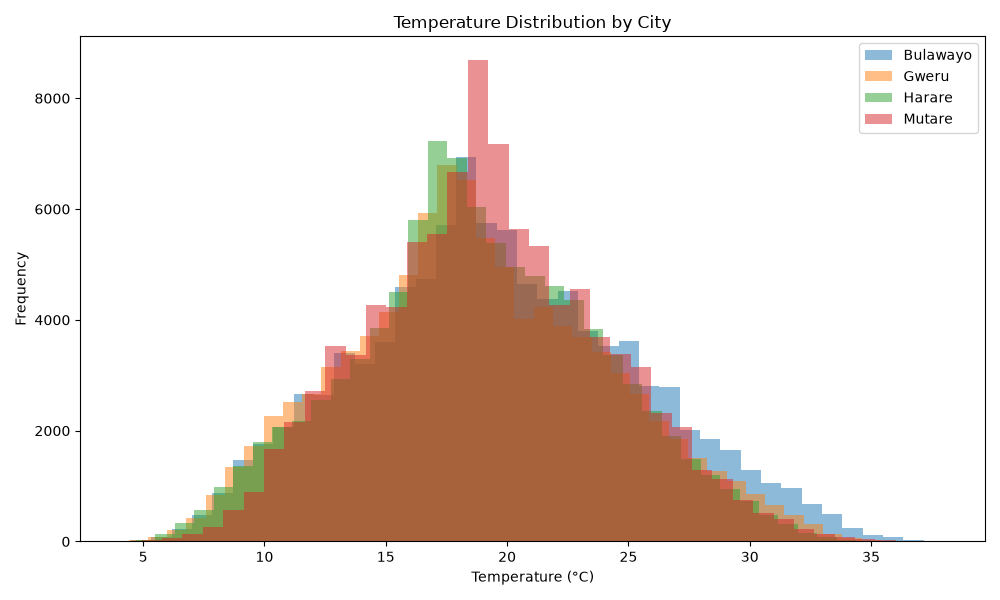
\includegraphics[width=0.9\textwidth]{temperature_distribution_by_city.png}
		\caption{Distribution of historical hourly temperatures across
			Harare, Bulawayo, Mutare, and Gweru, 2015--2025.}
		\label{fig:temperature-distribution}
	\end{figure}
	
	\subsubsection{Annual Temperature Patterns}
	
	Figure~\ref{fig:annual-temperature} compares annual average
	temperatures across the four cities from 2015 to 2025. The plotted
	series show broadly synchronized year-to-year movement: cooler
	values appear around 2017 and 2022, followed by a rise through 2023
	and 2024, and a modest decrease in 2025. In the chart, 2024 is the
	warmest year in the displayed period for each city; Bulawayo reaches
	an annual average of approximately $20.8^\circ\mathrm{C}$. The
	city-level averages also suggest a relative warmth ordering in which
	Bulawayo is warmest overall, followed by Mutare, Harare, and Gweru.
	These rankings describe the annual averages shown in this dataset
	and should not be assumed to hold for every hour, season, or year.
	
	The similar timing of the rises and dips suggests that the cities
	share broad temporal influences, while differences in their average
	levels indicate that location still matters. However, an eleven-year
	plot alone cannot establish a long-term climate-change trend or
	identify a cause for particular warm or cool years. Explanations
	involving large-scale climate drivers such as El Ni\~no or La Ni\~na
	would require additional evidence and are not tested by this figure.
	
	\begin{figure}[H]
		\centering
		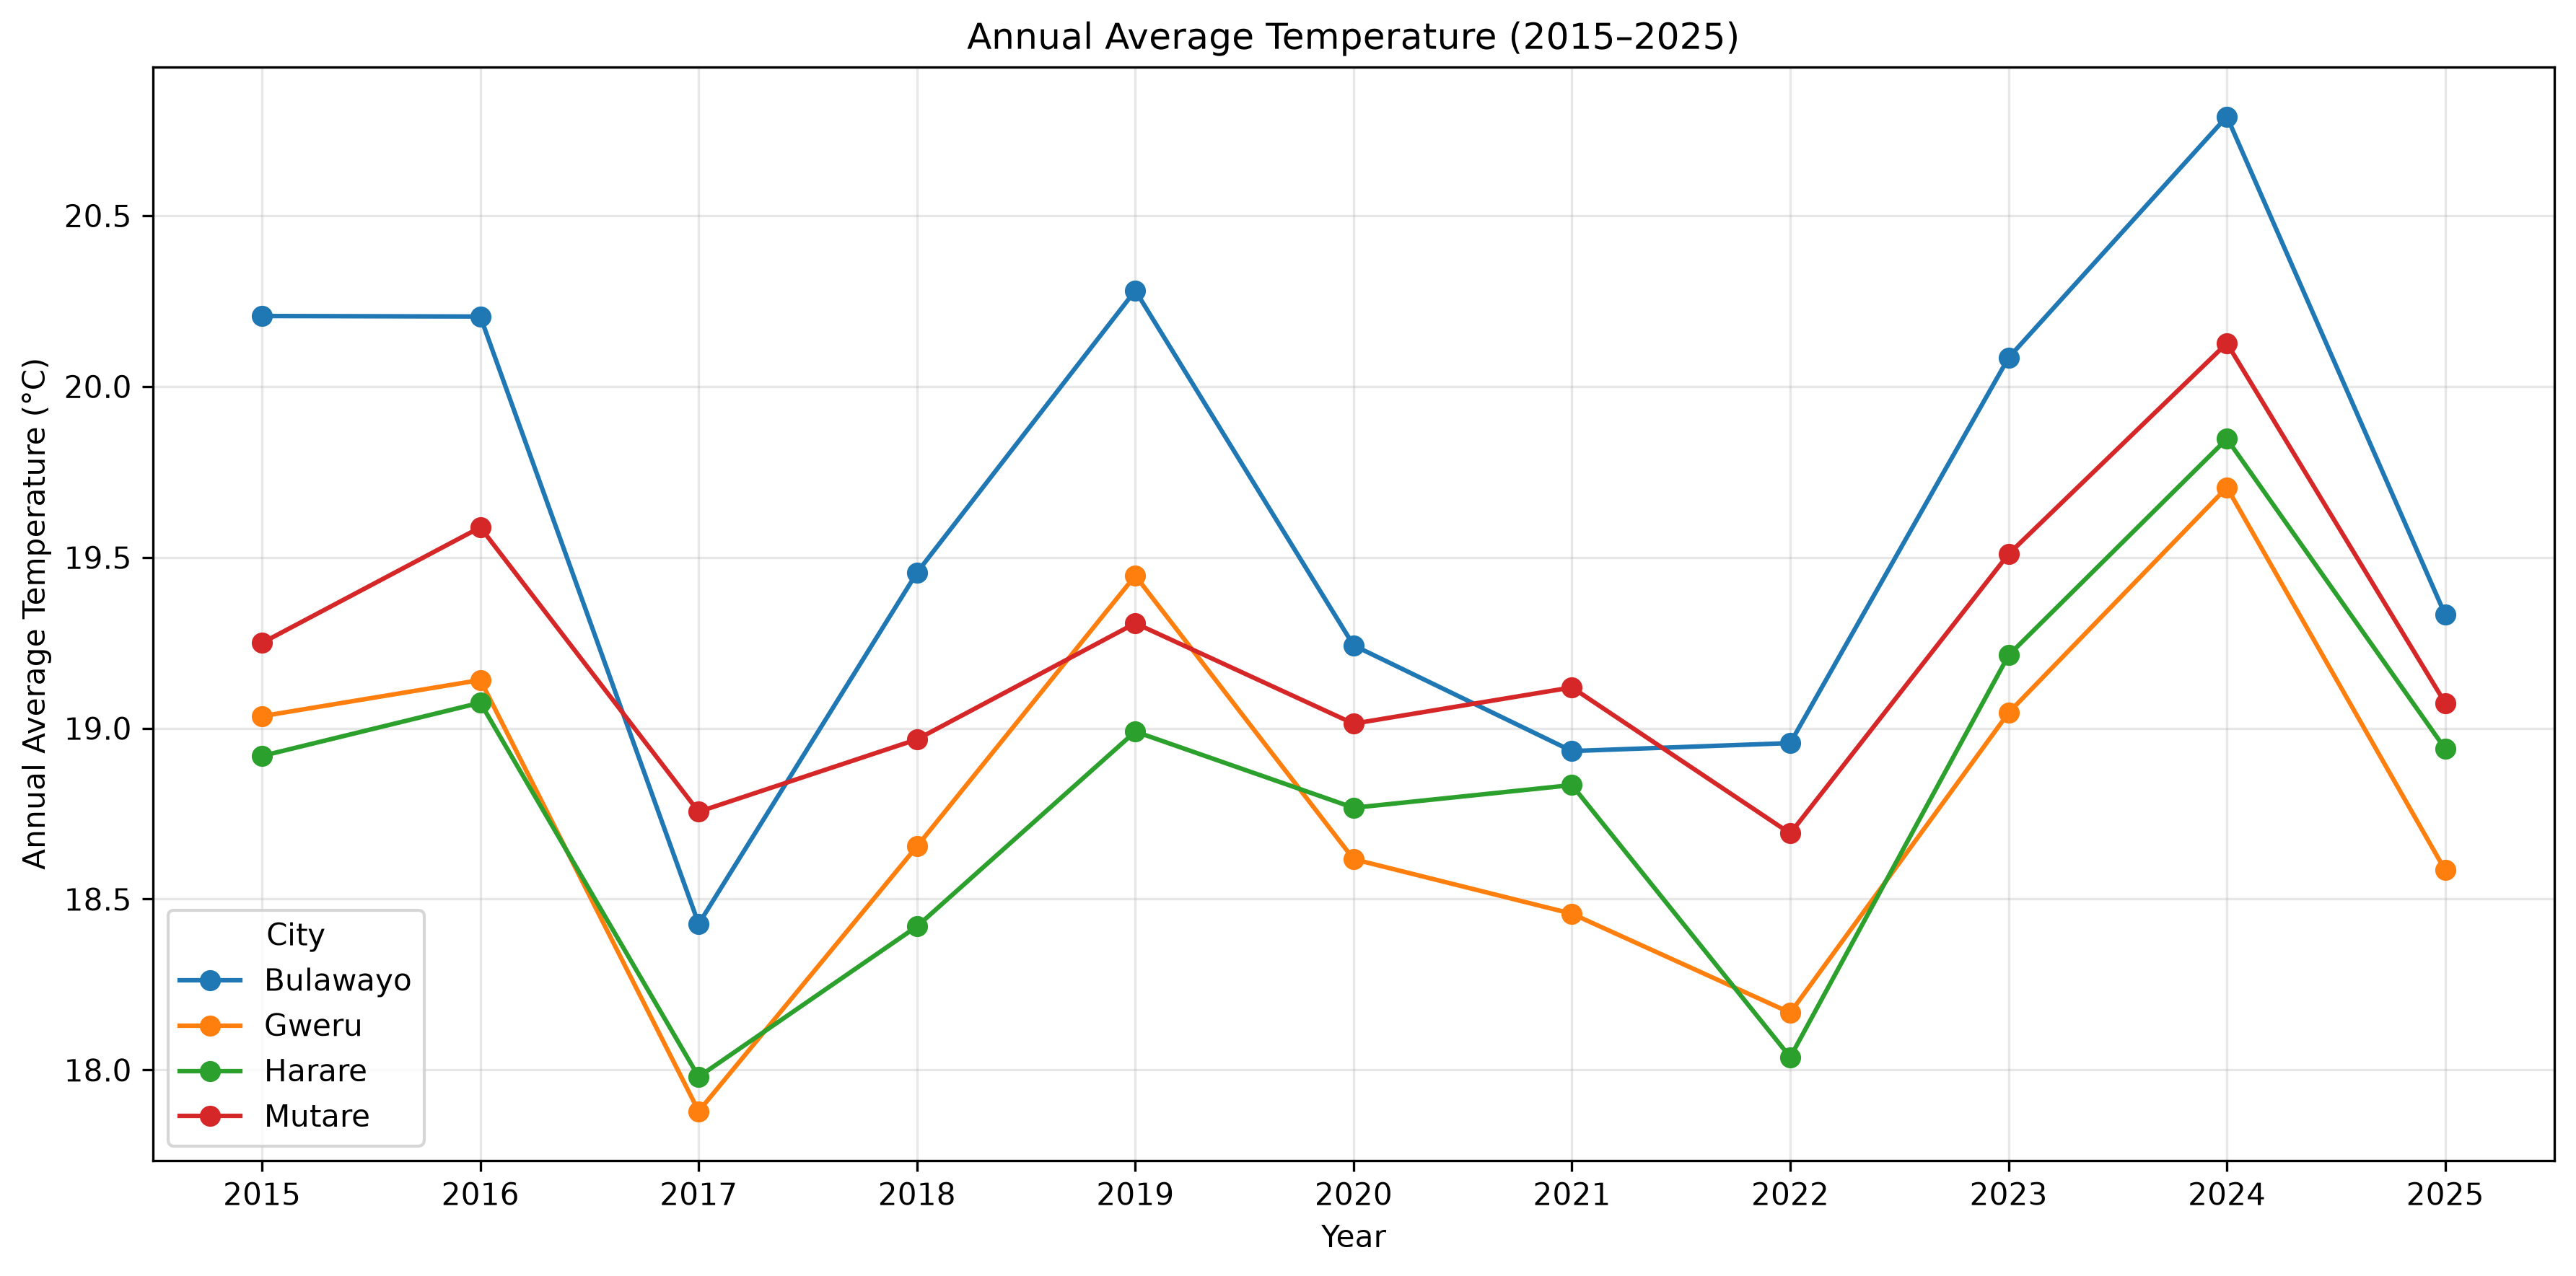
\includegraphics[width=0.9\textwidth]{annual_temperature_trend.png}
		\caption{Annual average temperature patterns across the four
			Zimbabwean cities, 2015--2025.}
		\label{fig:annual-temperature}
	\end{figure}
	
	\subsubsection{Average Monthly Temperature Patterns}
	
	Figure~\ref{fig:monthly-temperature} summarises the average monthly
	temperature cycle across the same period. The curves show clear
	seasonality consistent with Zimbabwe's Southern Hemisphere setting:
	averages are lowest during the winter months of June and July and
	rise towards the late dry-season and early summer period. Gweru has
	the lowest displayed July average, at approximately
	$14.0^\circ\mathrm{C}$, whereas Bulawayo reaches approximately
	$22.8^\circ\mathrm{C}$ around October. The chart also shows Mutare
	remaining warmer than Gweru during the coldest months. This
	separation indicates that the seasonal temperature profile differs
	by city, so a single national monthly average could conceal relevant
	local variation.
	
	Temperatures moderate after the October--November warm period in
	the plotted monthly averages, extending into the summer rainfall
	season. Cloud cover and precipitation may contribute to this
	pattern, but the monthly chart alone cannot isolate their effects.
	The annual and monthly summaries therefore provide complementary
	information: annual averages show year-to-year variation, while
	monthly averages reveal the recurring seasonal cycle. Both support
	including temporal information and city identity in the prediction
	workflow, while the forecasting models must be assessed using the
	chronological validation and test periods described below.
	
	\begin{figure}[H]
		\centering
		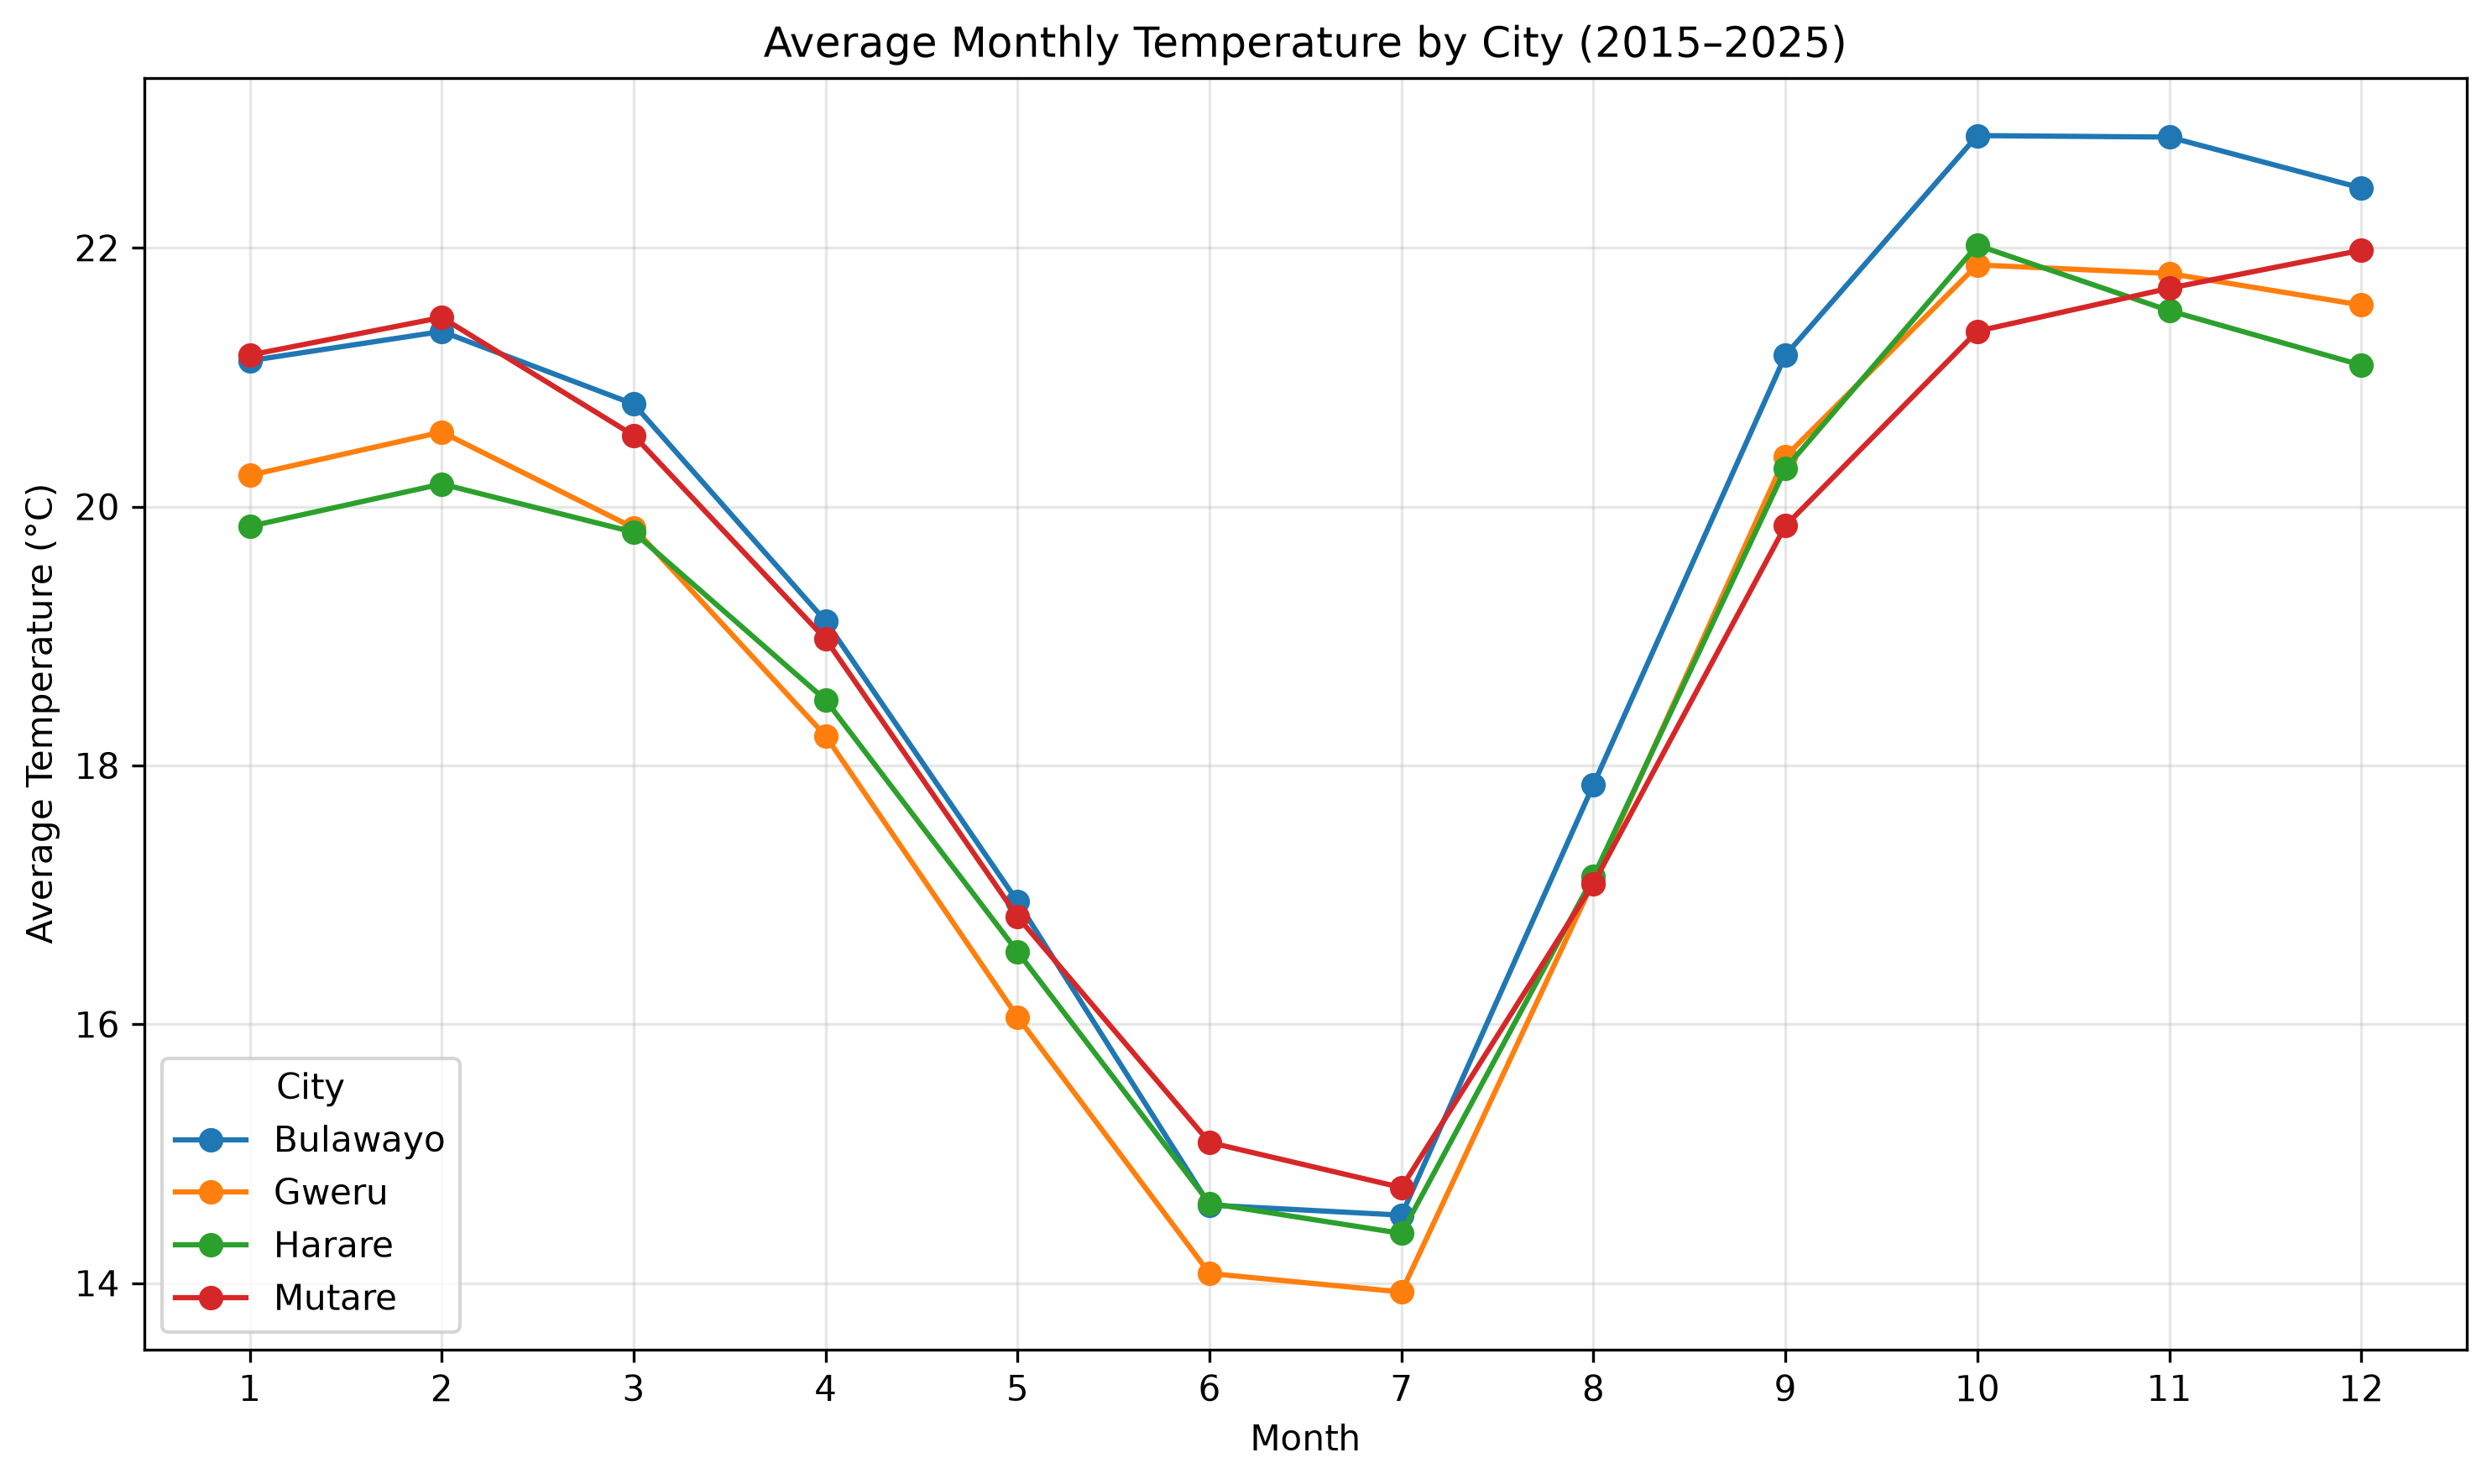
\includegraphics[width=0.9\textwidth]{average_monthly_temperature.png}
		\caption{Average monthly temperature patterns across Harare,
			Bulawayo, Mutare, and Gweru, aggregated over 2015--2025.}
		\label{fig:monthly-temperature}
	\end{figure}
	
	\subsubsection{Weather-Variable Correlations}
	
	Figure~\ref{fig:weather-correlation} presents the Pearson correlation
	matrix for seven meteorological variables: air temperature
	(\texttt{temperature\_2m}), relative humidity
	(\texttt{relative\_humidity\_2m}), precipitation, mean sea-level
	pressure (\texttt{pressure\_msl}), wind speed
	(\texttt{wind\_speed\_10m}), wind direction, and cloud cover.
	Pearson's correlation coefficient measures the direction and strength
	of a pairwise linear association. Correlation summaries are descriptive
	statistics and should be interpreted in the context of the underlying
	data and analysis design \cite{wilks2019}. Values range from $-1$ to $+1$:
	values close to $+1$ indicate strong positive associations, values
	close to $-1$ indicate strong negative associations, and values near
	zero indicate weak linear associations. Correlation does not establish
	that one variable causes changes in another.
	
	The coefficients displayed in Figure~\ref{fig:weather-correlation}
	show several relationships among the recorded weather variables.
	Temperature has a negative correlation with mean sea-level pressure
	($r=-0.68$) and relative humidity ($r=-0.58$), indicating that higher
	temperature observations tend to occur alongside lower values of these
	variables in this dataset. Relative humidity has a moderate positive
	correlation with cloud cover ($r=0.44$), suggesting that higher
	humidity observations tend to coincide with greater cloud cover.
	Wind speed has a weak positive correlation with mean sea-level pressure
	($r=0.22$), while its correlations with temperature and relative
	humidity are close to zero ($r=-0.04$ and $r=-0.03$, respectively).
	These coefficients describe associations in the observations; they
	do not, by themselves, establish the physical mechanisms responsible
	for the relationships.
	
	Precipitation exhibits weak linear correlations across the variables
	in the matrix, ranging from $r=-0.12$ with pressure to $r=0.20$ with
	cloud cover. Precipitation can be intermittent and highly skewed, with
	many observations potentially recording no rainfall. Consequently,
	weak Pearson correlations do not necessarily mean that precipitation
	is unrelated to other atmospheric conditions: nonlinear relationships
	or conditions associated with particular rainfall events may not be
	captured by a single linear coefficient.
	
	Wind direction requires particular care because it is an angular
	variable, where $0^\circ$ and $360^\circ$ represent the same direction.
	Ordinary Pearson correlation applied directly to raw direction
	degrees can therefore misrepresent its relationship with other
	variables. A more suitable approach for subsequent analysis may be
	to represent wind direction using sine and cosine components before
	examining relationships or including direction in model features.
	
	The correlation matrix is useful for exploratory analysis and for
	identifying potentially redundant predictors. However, high pairwise
	correlation does not automatically require feature removal. In linear
	models, multicollinearity can make individual coefficient estimates
	less stable. Tree-based models such as Random Forest and XGBoost can
	capture nonlinear relationships and interactions, although correlated
	predictors may share predictive information and affect how feature
	importance is distributed. Therefore, the matrix should guide further
	feature investigation rather than determine feature selection in
	isolation.
	
	\begin{figure}[H]
		\centering
		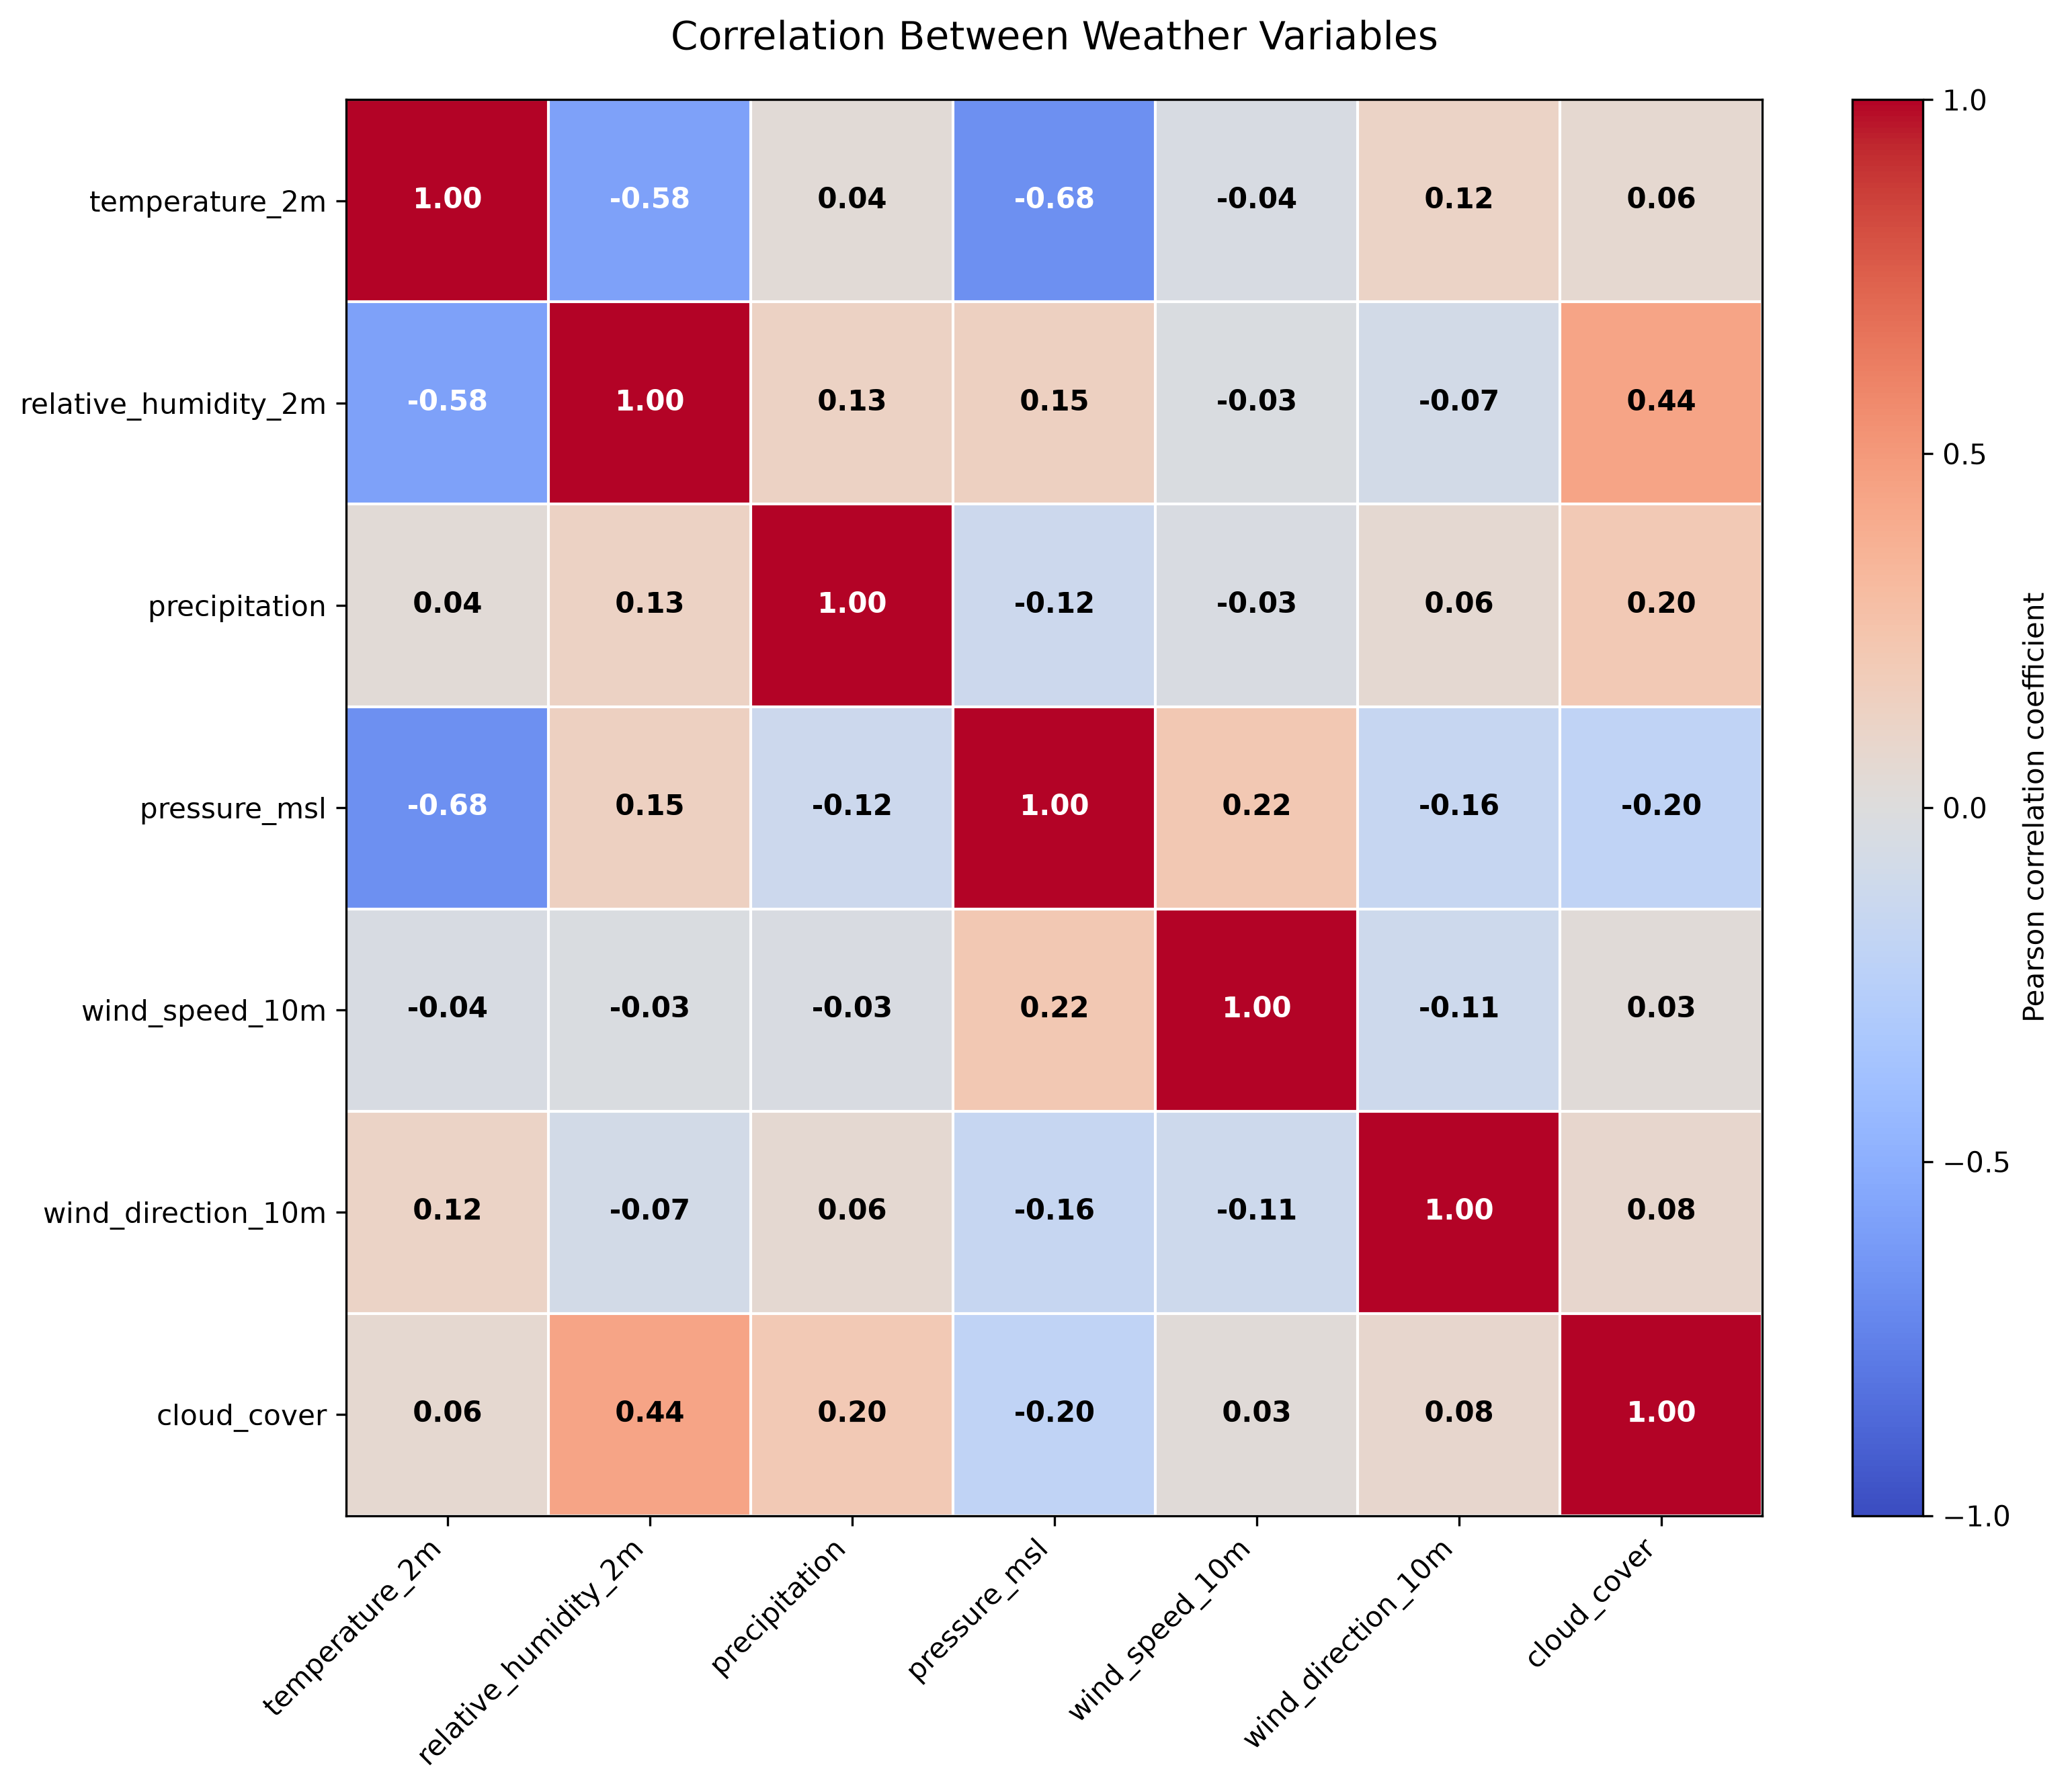
\includegraphics[width=0.9\textwidth]{weather_variable_correlation.png}
		\caption{Pearson correlation matrix for selected weather variables.
			Each cell displays the numerical coefficient to two decimal places;
			coefficients range from $-1$ to $+1$.}
		\label{fig:weather-correlation}
	\end{figure}
	\subsection{Feature Engineering}
	
	Feature engineering represented temporal structure and recent
	weather conditions. Features in the modelling workflow include
	current weather measurements, time-of-day representations,
	historical temperature lags, rolling temperature summaries, and
	other temporal indicators. The feature-importance output includes
	variables such as \texttt{temperature\_2m},
	\texttt{temperature\_lag\_24h}, \texttt{temperature\_lag\_1h},
	\texttt{hour\_sin}, and \texttt{hour\_cos}.
	
	For valid forecasting evaluation, each feature must be available
	at the time a prediction is made. Future target observations must
	not be used to construct input features. The exact feature list and
	the implementation of lag and rolling windows should be documented
	from the final feature-engineering script.
	
	\subsection{Prediction Target}
	
	The task is one-hour-ahead temperature prediction. Conceptually,
	the model estimates
	\begin{equation}
		\widehat{T}_{t+1}=f(X_t,X_{t-1},\ldots,X_{t-k}),
	\end{equation}
	where $\widehat{T}_{t+1}$ is the predicted temperature one hour
	ahead, $f$ is the fitted model, and the $X$ terms represent
	observations and engineered features available at prediction time.
	The precise value of $k$ depends on the features used in the final
	pipeline.
	
	\subsection{Chronological Data Splitting}
	
	The data were split chronologically, as summarised in
	Table~\ref{tab:temporal-split}.
	
	\begin{table}[H]
		\centering
		\caption{Temporal evaluation strategy}
		\label{tab:temporal-split}
		\begin{tabular}{ll}
			\toprule
			\textbf{Subset} & \textbf{Period}\\
			\midrule
			Training & Data through 2022\\
			Validation & 2023--2024\\
			Testing & 2025\\
			\bottomrule
		\end{tabular}
	\end{table}
	
	The training period was used to fit model parameters, validation
	data supported development and model-selection decisions, and the
	test period was used for the reported final comparison, consistent
	with the principle that forecast accuracy should be assessed on data
	not used to fit the model \cite{hyndman2021,bergmeir2018}. This design
	reflects the temporal ordering of the task better than an
	unrestricted random split. Preprocessing, lag construction, scaling,
	and hyperparameter selection must also respect temporal boundaries
	to avoid leakage.
	
	\subsection{Candidate Models}
	
	Six approaches were evaluated:
	\begin{itemize}[leftmargin=*]
		\item \textbf{Persistence baseline:} uses the most recent
		observed temperature as the next-temperature estimate.
		\item \textbf{Linear Regression:} models the target as a linear
		function of the selected features.
		\item \textbf{Random Forest:} combines decision trees to model
		nonlinear relationships.
		\item \textbf{XGBoost:} uses gradient-boosted trees to learn
		patterns in the engineered features.
		\item \textbf{Baseline LSTM:} uses a recurrent neural network
		to model sequential patterns.
		\item \textbf{Improved LSTM v2:} represents a revised LSTM
		experiment intended to improve on the baseline sequence model.
	\end{itemize}
	Detailed hyperparameters, sequence length, scaling procedures, and
	training configurations should be recorded from the actual
	experiment scripts and logs.
	
	% --------------------------------------------------
	% EXPLORATORY SATELLITE ANALYSIS
	% --------------------------------------------------
	\subsection{Exploratory Sentinel-2 Satellite Analysis}
	
	A separate exploratory satellite analysis was conducted over a small
	area around Harare to investigate how multispectral imagery can support
	environmental surface-change screening. This experiment is distinct
	from the weather modelling pipeline: satellite-derived indices were
	not used as features in the deployed XGBoost temperature prediction
	model, and the satellite outputs do not affect the model metrics
	reported in this study.
	
	Sentinel-2 imagery, collected by the multispectral imaging mission
	described by Drusch et al. (2012)\cite{drusch2012}, was examined for
	12 October 2025 and 19 October 2025 using imagery accessed through the
	Copernicus Data Space Ecosystem \cite{copernicusdataspace}, over the approximate bounding box
	$[31.00,-17.90,31.10,-17.75]$. Candidate scenes were selected using
	a cloud-cover threshold below 20\%. The reference scene metadata for
	19 October 2025 identifies Sentinel-2A and an acquisition time of
	11:14:13 UTC. The raster products generated for the experiment are
	1000 by 1000 pixels. Their metadata indicates a nominal 10 m pixel
	spacing; however, the coordinate reference system, raster alignment,
	and pixel-area assumptions must be verified before mapped areas are
	treated as definitive.
	
	The Normalized Difference Vegetation Index (NDVI), a widely used spectral
	indicator for vegetation monitoring \cite{tucker1979}, was calculated as
	\begin{equation}
		\mathrm{NDVI}=\frac{\mathrm{NIR}-\mathrm{Red}}
		{\mathrm{NIR}+\mathrm{Red}},
	\end{equation}
	where the near-infrared and red bands represent vegetation reflectance.
	The Normalized Burn Ratio (NBR) was calculated using Sentinel-2 band
	B08 as near-infrared and B12 as short-wave infrared:
	\begin{equation}
		\mathrm{NBR}=\frac{B08-B12}{B08+B12}.
	\end{equation}
	The differenced NBR (dNBR), commonly used in post-fire severity
	assessment but not uniquely diagnostic of fire \cite{keybenson2006}, was calculated as the NBR for
	12 October minus the NBR for 19 October 2025:
	\begin{equation}
		\mathrm{dNBR}=\mathrm{NBR}_{12\,\mathrm{Oct}}
		-\mathrm{NBR}_{19\,\mathrm{Oct}}.
	\end{equation}
	Under this sign convention, positive dNBR values indicate a reduction
	in NBR between the two dates. Such a reduction can be associated with
	surface or vegetation changes, but it is not specific to fire and
	cannot independently confirm a burn event.
	
	For exploratory visualisation, dNBR values were assigned to four
	classes: high positive change ($\mathrm{dNBR}\geq0.20$), moderate
	positive change ($0.10\leq\mathrm{dNBR}<0.20$), little or no change
	($-0.10\leq\mathrm{dNBR}<0.10$), and negative change
	($\mathrm{dNBR}<-0.10$). Connected candidate high-change regions were
	then identified from pixels with dNBR at least 0.20 using 8-neighbour
	connectivity. Regions containing fewer than 10 pixels were excluded
	from the retained-region summary. These thresholds are exploratory
	screening choices, not a locally validated fire-severity classification.
	
	\subsection{Evaluation Metrics}
	
	\subsubsection{Mean Absolute Error}
	
	Mean Absolute Error (MAE) measures the average absolute difference
	between predicted and observed values:
	\begin{equation}
		\mathrm{MAE}=\frac{1}{n}\sum_{i=1}^{n}|y_i-\widehat{y}_i|.
	\end{equation}
	Here, $y_i$ is the observed temperature, $\widehat{y}_i$ is the
	predicted temperature, and $n$ is the number of test observations.
	Lower MAE indicates smaller average absolute errors. This metric is
	commonly used to summarise regression prediction errors \cite{scikitlearnmetrics}.
	
	\subsubsection{Root Mean Squared Error}
	
	Root Mean Squared Error (RMSE) is defined as
	\begin{equation}
		\mathrm{RMSE}=\sqrt{\frac{1}{n}\sum_{i=1}^{n}
			(y_i-\widehat{y}_i)^2}.
	\end{equation}
	RMSE gives greater weight to larger errors than MAE. Lower values
	indicate better performance \cite{scikitlearnmetrics}.
	
	\subsubsection{Coefficient of Determination}
	
	The coefficient of determination is calculated as
	\begin{equation}
		R^2=1-\frac{\sum_{i=1}^{n}(y_i-\widehat{y}_i)^2}
		{\sum_{i=1}^{n}(y_i-\bar{y})^2},
	\end{equation}
	where $\bar{y}$ is the mean of the observed test values. Higher
	values generally indicate that predictions account for a greater
	proportion of variation in the test targets. $R^2$ should be
	interpreted alongside error metrics and the evaluation dataset.
	
	% --------------------------------------------------
	% 4. RESULTS
	% --------------------------------------------------
	\section{Results}
	
	\subsection{Dataset Preparation}
	
	The consolidated dataset contained 385,728 hourly records across
	the four study cities for 2015--2025. The preprocessing checks
	reported no missing values and no duplicate records in the prepared
	dataset. Additional timestamp-continuity and variable-range checks
	remain useful for reproducibility and quality assurance.
	
	\subsection{Model Performance Comparison}
	
	Table~\ref{tab:model-comparison} presents the reported test metrics
	for all six evaluated approaches.
	
	\begin{table}[htbp]
		\centering
		\caption{Model performance on the 2025 test dataset}
		\label{tab:model-comparison}
		\small
		\begin{tabular}{lrrr}
			\toprule
			\textbf{Model} & \textbf{MAE ($^\circ$C)} &
			\textbf{RMSE ($^\circ$C)} & \textbf{$R^2$}\\
			\midrule
			Persistence       & 0.9090 & 1.2067 & 0.9367\\
			Linear Regression & 0.4745 & 0.7038 & 0.9785\\
			Random Forest     & 0.3477 & 0.5349 & 0.9876\\
			XGBoost           & 0.3448 & 0.5210 & 0.9882\\
			Baseline LSTM     & 0.8016 & 1.0334 & 0.9536\\
			Improved LSTM v2 & 0.7771 & 1.0002 & 0.9565\\
			\bottomrule
		\end{tabular}
	\end{table}
	
	XGBoost achieved the lowest reported MAE and RMSE and the highest
	reported $R^2$ among the evaluated models. Its MAE was
	0.3448$^\circ$C, its RMSE was 0.5210$^\circ$C, and its $R^2$ was
	0.9882. Random Forest performed closely, with an MAE of
	0.3477$^\circ$C. The absolute difference in MAE between XGBoost and
	Random Forest was 0.0029$^\circ$C. Linear Regression outperformed
	the persistence baseline, while both LSTM experiments had higher
	errors than the two tree-based ensemble methods in this comparison.
	
	Figure~\ref{fig:model-comparison-mae} provides a visual comparison
	of the six models using MAE. The table provides the exact reported
	metrics, while the figure makes the relative MAE differences easier
	to compare. Together, the results support selecting XGBoost for the
	current deployed system, while not proving that it will outperform
	all alternative approaches on other datasets, locations, or horizons.
	
	\begin{figure}[H]
		\centering
		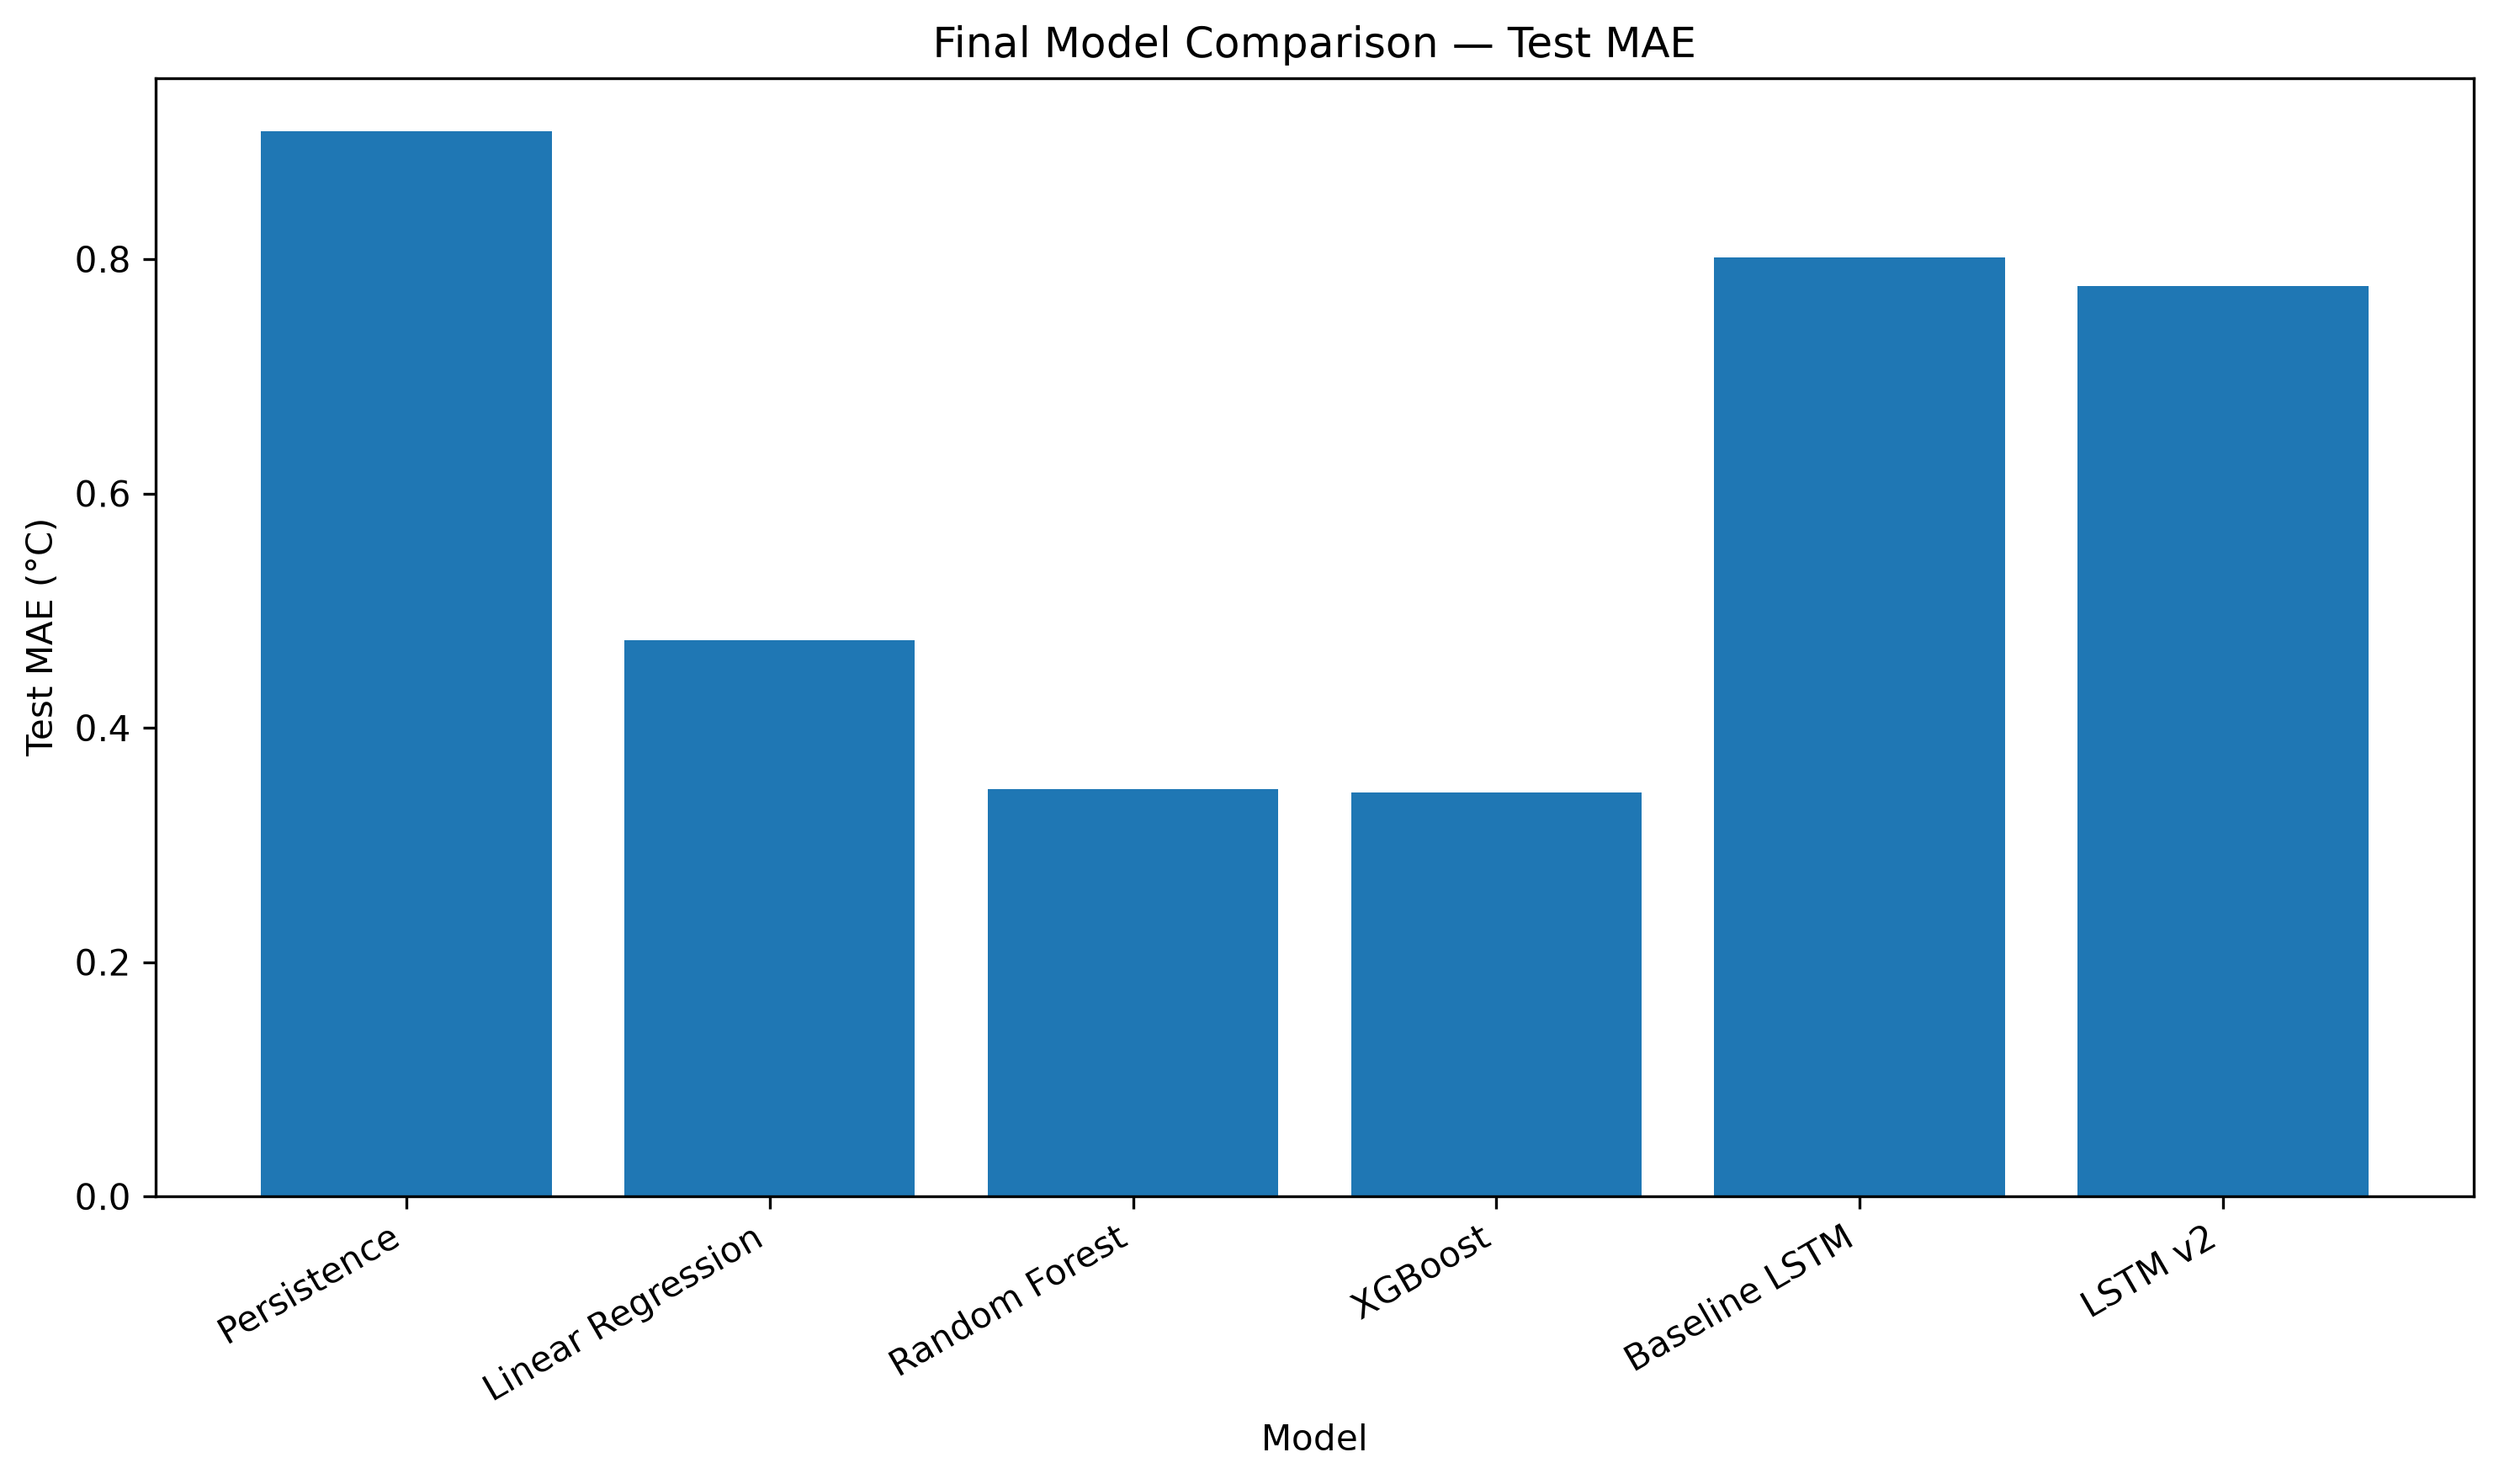
\includegraphics[width=0.9\textwidth]{final_model_comparison_mae.png}
		\caption{Comparison of candidate models using MAE on the test
			dataset. Lower values indicate smaller average absolute errors.}
		\label{fig:model-comparison-mae}
	\end{figure}
	
	\subsection{Feature Importance}
	
	The XGBoost feature-importance output identified current temperature
	(\texttt{temperature\_2m}) as the most influential feature, with an
	importance value of approximately 0.6645 (66.45\%). The
	24-hour temperature lag (\texttt{temperature\_lag\_24h}) had an
	importance value of approximately 0.1783 (17.83\%). Together, these
	two features account for approximately 84.28\% of the reported
	importance values.
	
	Other contributing features included cyclical hour features,
	the one-hour temperature lag, and rolling temperature statistics.
	Figure~\ref{fig:xgboost-importance} presents the feature-importance
	visualisation generated by the project.
	
	These values describe importance under the method used by the
	trained model; they do not establish causal effects. Their
	interpretation also depends on the importance measure and
	correlations between features. The final report should identify the
	specific importance method used by the script if it is available.
	
	\begin{figure}[H]
		\centering
		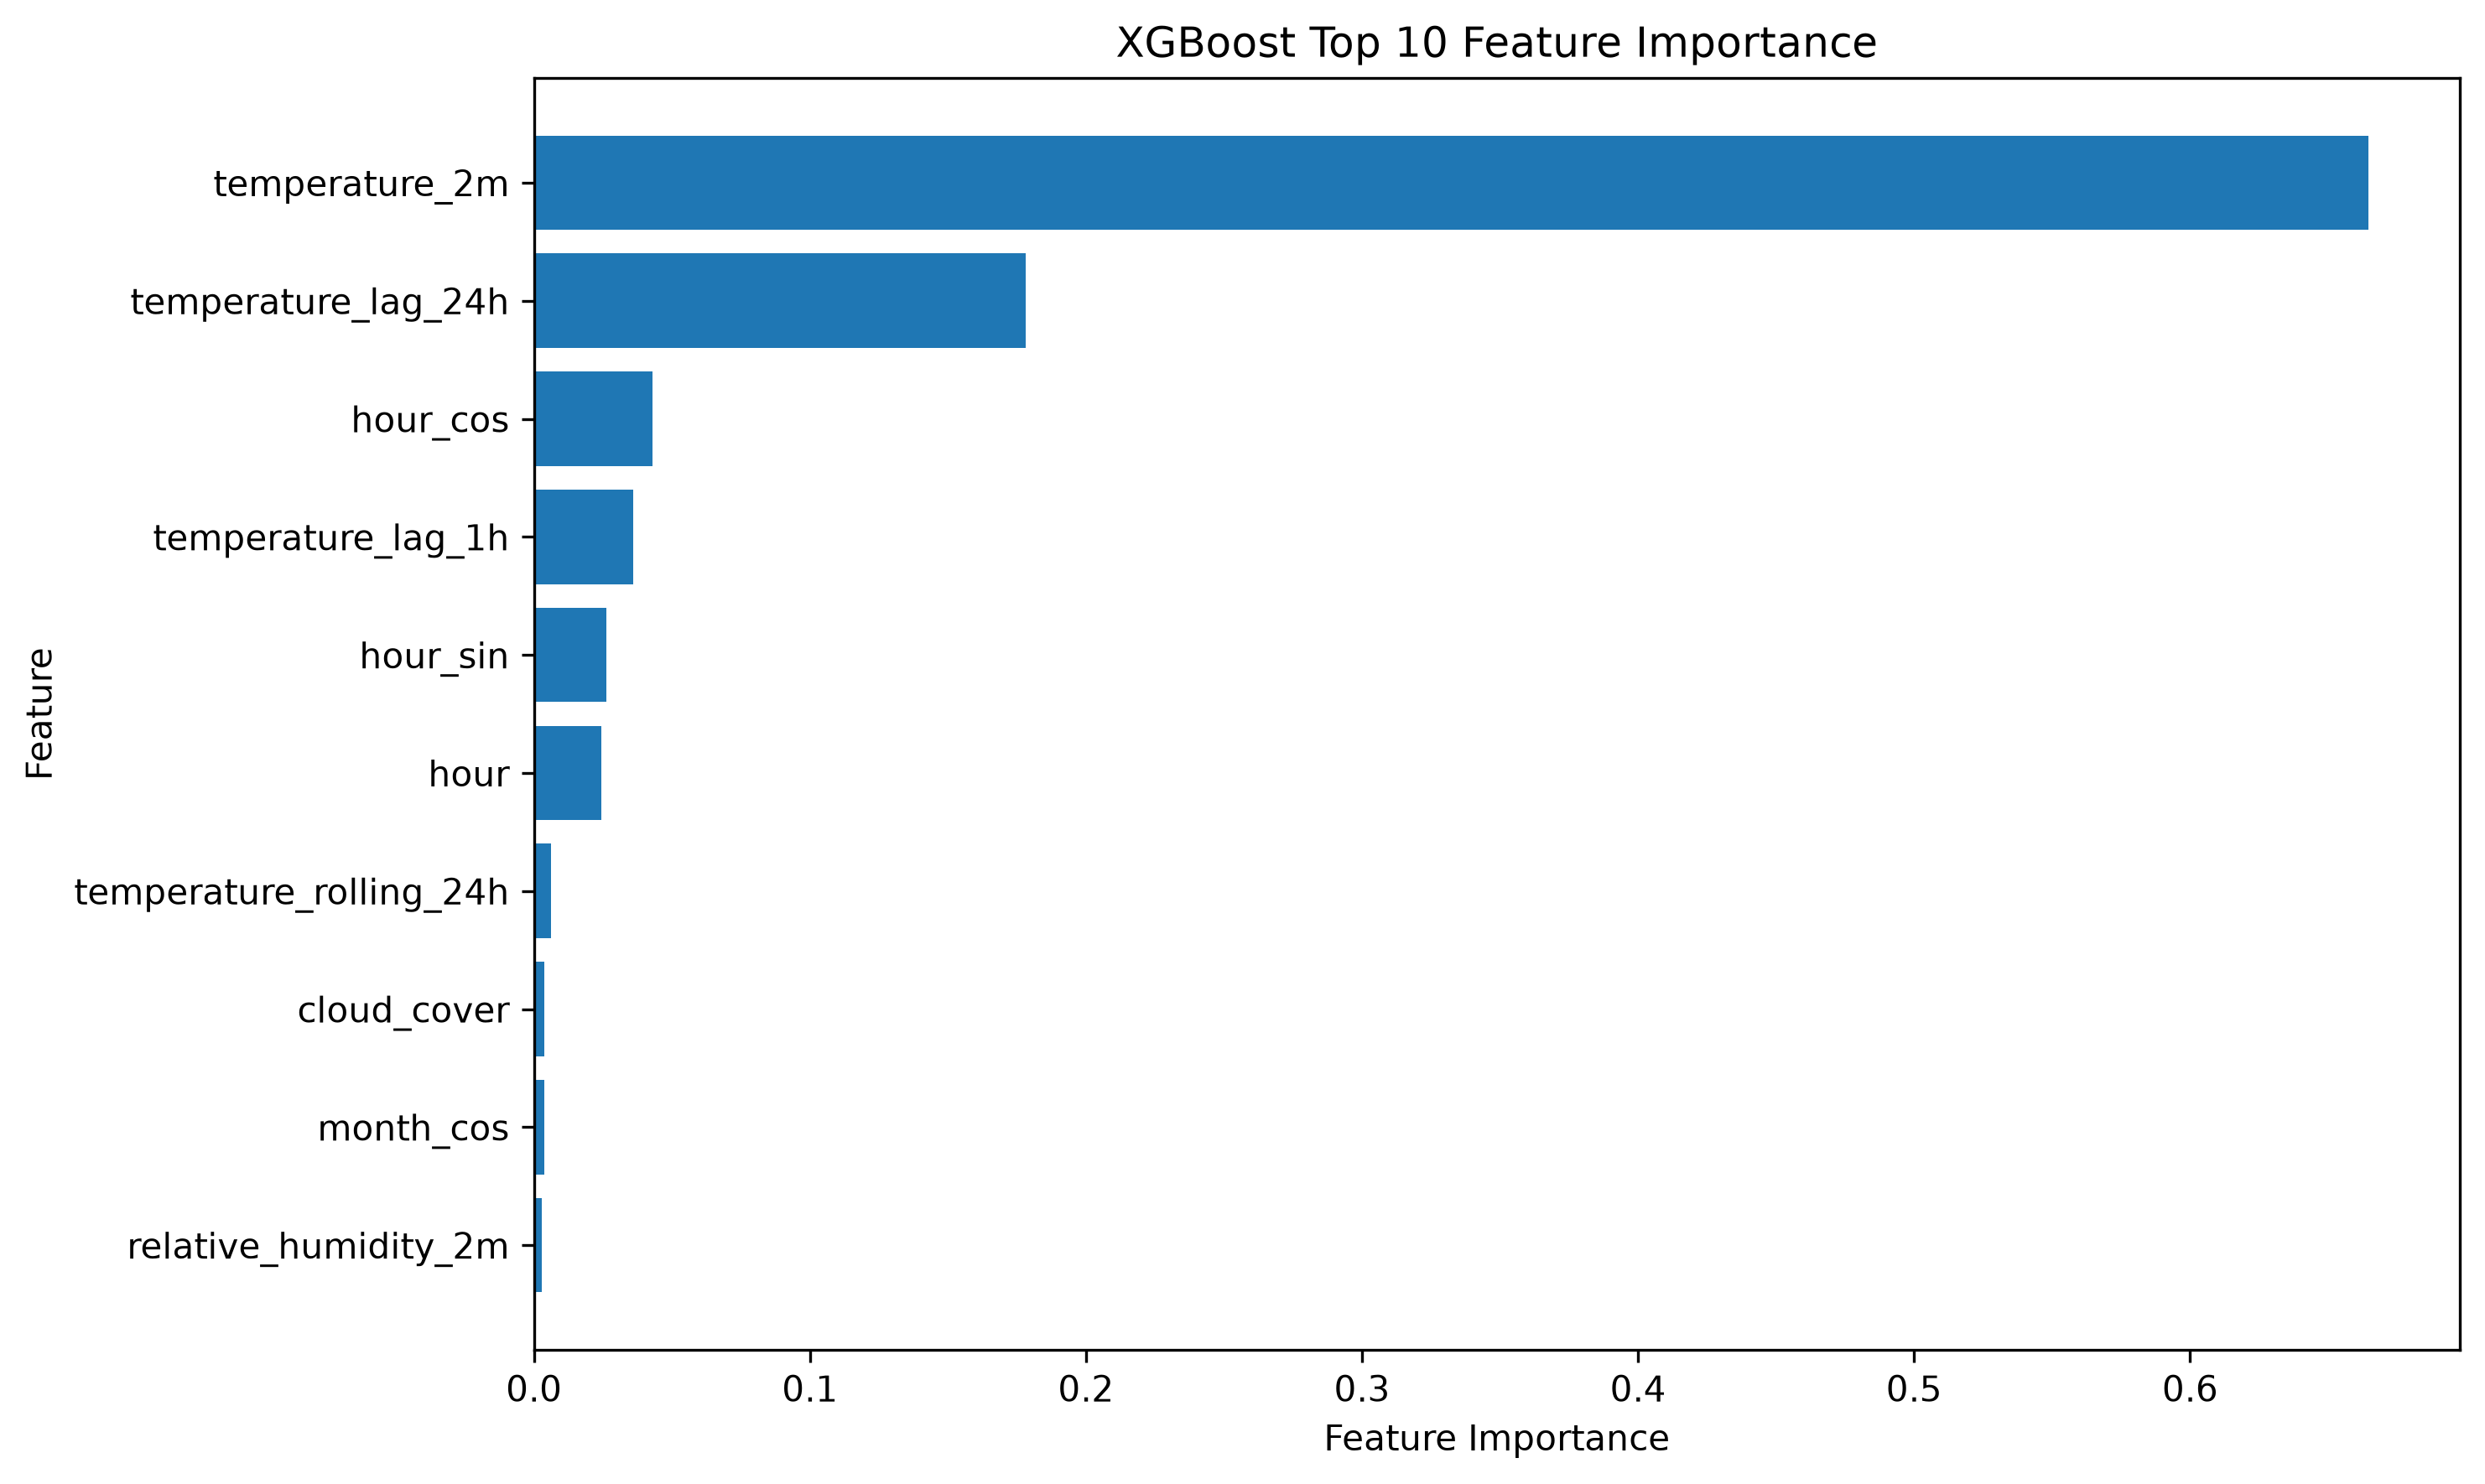
\includegraphics[width=0.9\textwidth]{xgboost_feature_importance.png}
		\caption{Feature importance for the selected XGBoost temperature
			prediction model.}
		\label{fig:xgboost-importance}
	\end{figure}
	
	% --------------------------------------------------
	% SATELLITE EXPERIMENT RESULTS
	% --------------------------------------------------
	\subsection{Exploratory Satellite Results for Harare}
	
	The satellite experiment produced a true-colour Sentinel-2 image,
	vegetation and Normalized Burn Ratio (NBR) index maps, a vegetation
	mask, a continuous differenced Normalized Burn Ratio (dNBR) map, a
	classified dNBR map, and a filtered map of connected candidate
	high-change regions. These outputs describe the exploratory satellite
	workflow only. They are standalone environmental diagnostics and are
	not inputs to, or outputs of, the deployed temperature-prediction
	service.
	
	\subsubsection{Land Cover and Vegetation Indices}
	
	\begin{figure}[H]
		\centering
		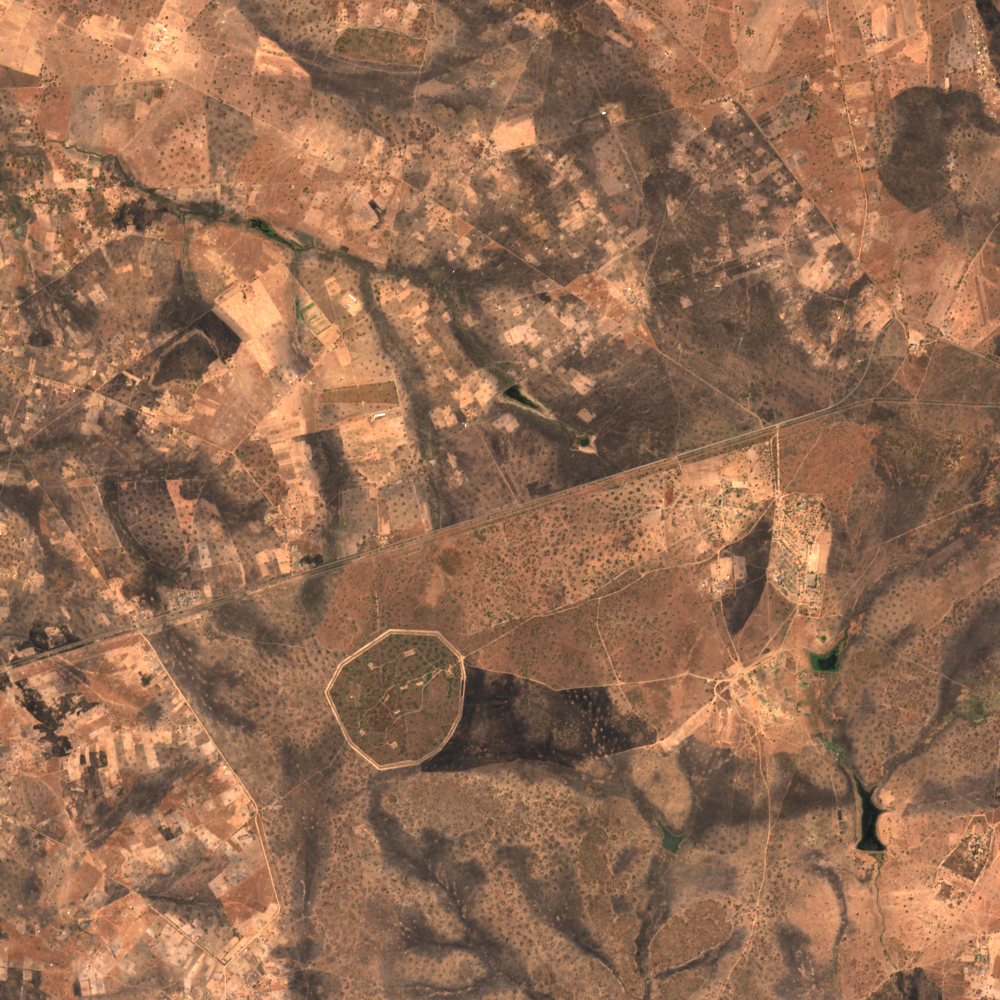
\includegraphics[width=0.88\textwidth]{harare_sentinel2_tci_20251019.png}
		\caption{Sentinel-2A true-colour image for the Harare study area,
			acquired on 19 October 2025.}
		\label{fig:harare-sentinel2-tci}
	\end{figure}
	
	Figure~\ref{fig:harare-sentinel2-tci} provides visual context for the
	landscape and its visible land-surface patterns. Although the image
	can help identify areas for further inspection, visual appearance
	alone is insufficient to determine whether a dark surface feature
	represents burning, harvesting, exposed soil, shadow, or another
	land-cover condition.
	
	\begin{figure}[H]
		\centering
		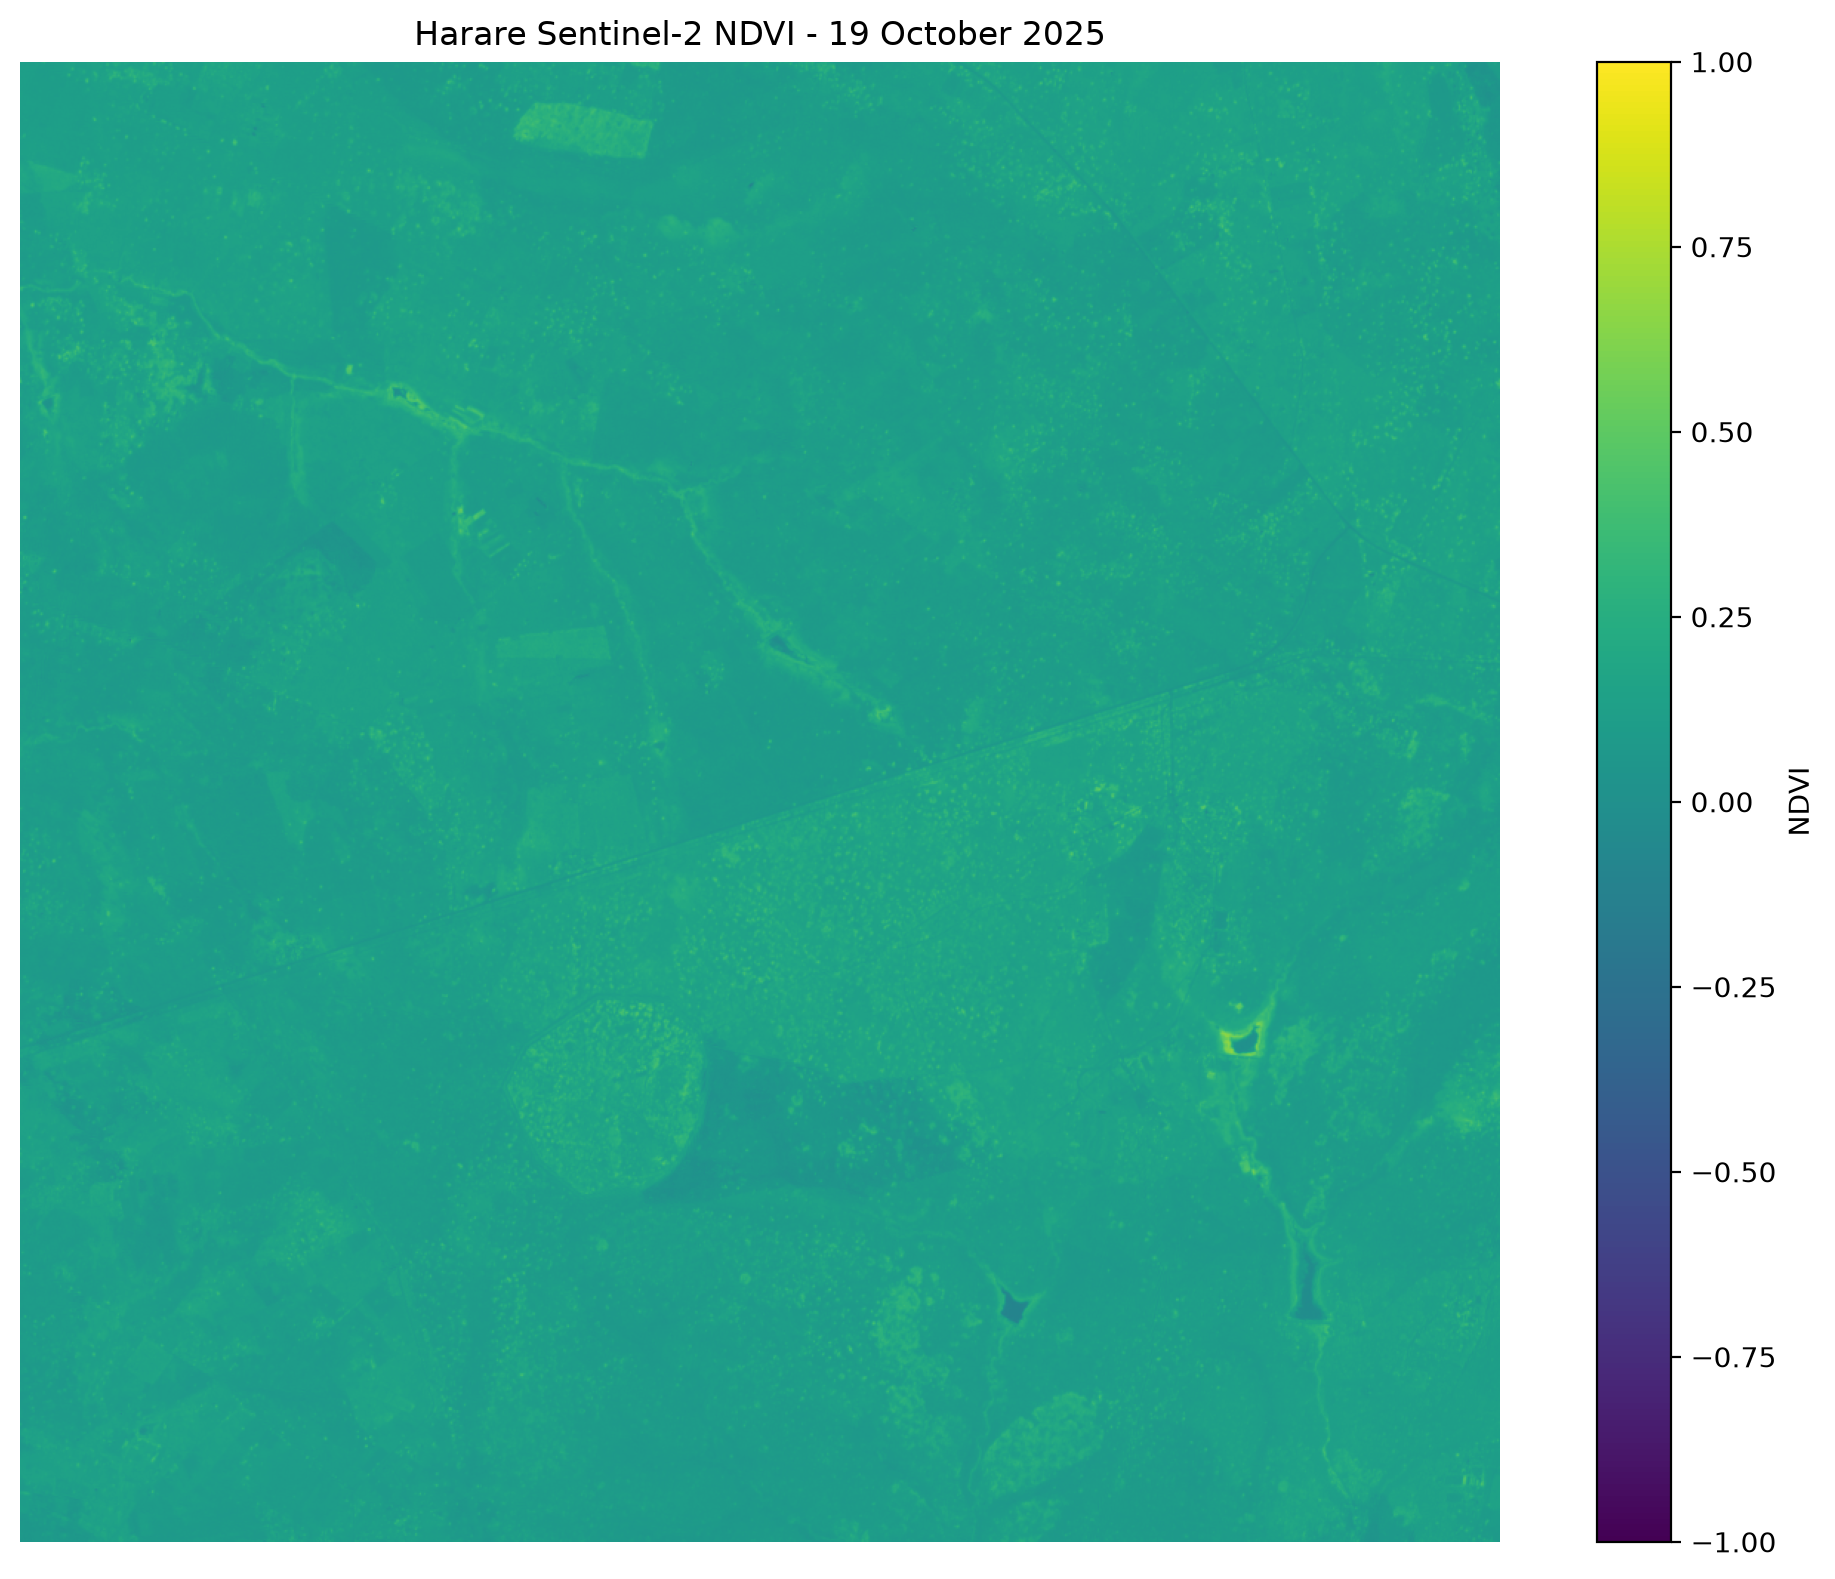
\includegraphics[width=0.82\textwidth]{harare_ndvi_map_20251019.png}
		\caption{NDVI map derived from the Sentinel-2 image for
			19 October 2025.}
		\label{fig:harare-ndvi}
	\end{figure}
	
	The Normalized Difference Vegetation Index (NDVI) raster contained
	999,997 valid pixels, with a minimum of $-0.1157$, maximum of
	$0.6595$, mean of $0.1282$, and median of $0.1216$. A total of 3,929
	valid pixels had NDVI greater than 0.30, approximately 0.39\% of the
	valid pixels. This threshold-based count is a descriptive index
	summary rather than a definitive vegetation inventory; interpretation
	also depends on masking, land-cover conditions, and local validation.
	
	\begin{figure}[H]
		\centering
		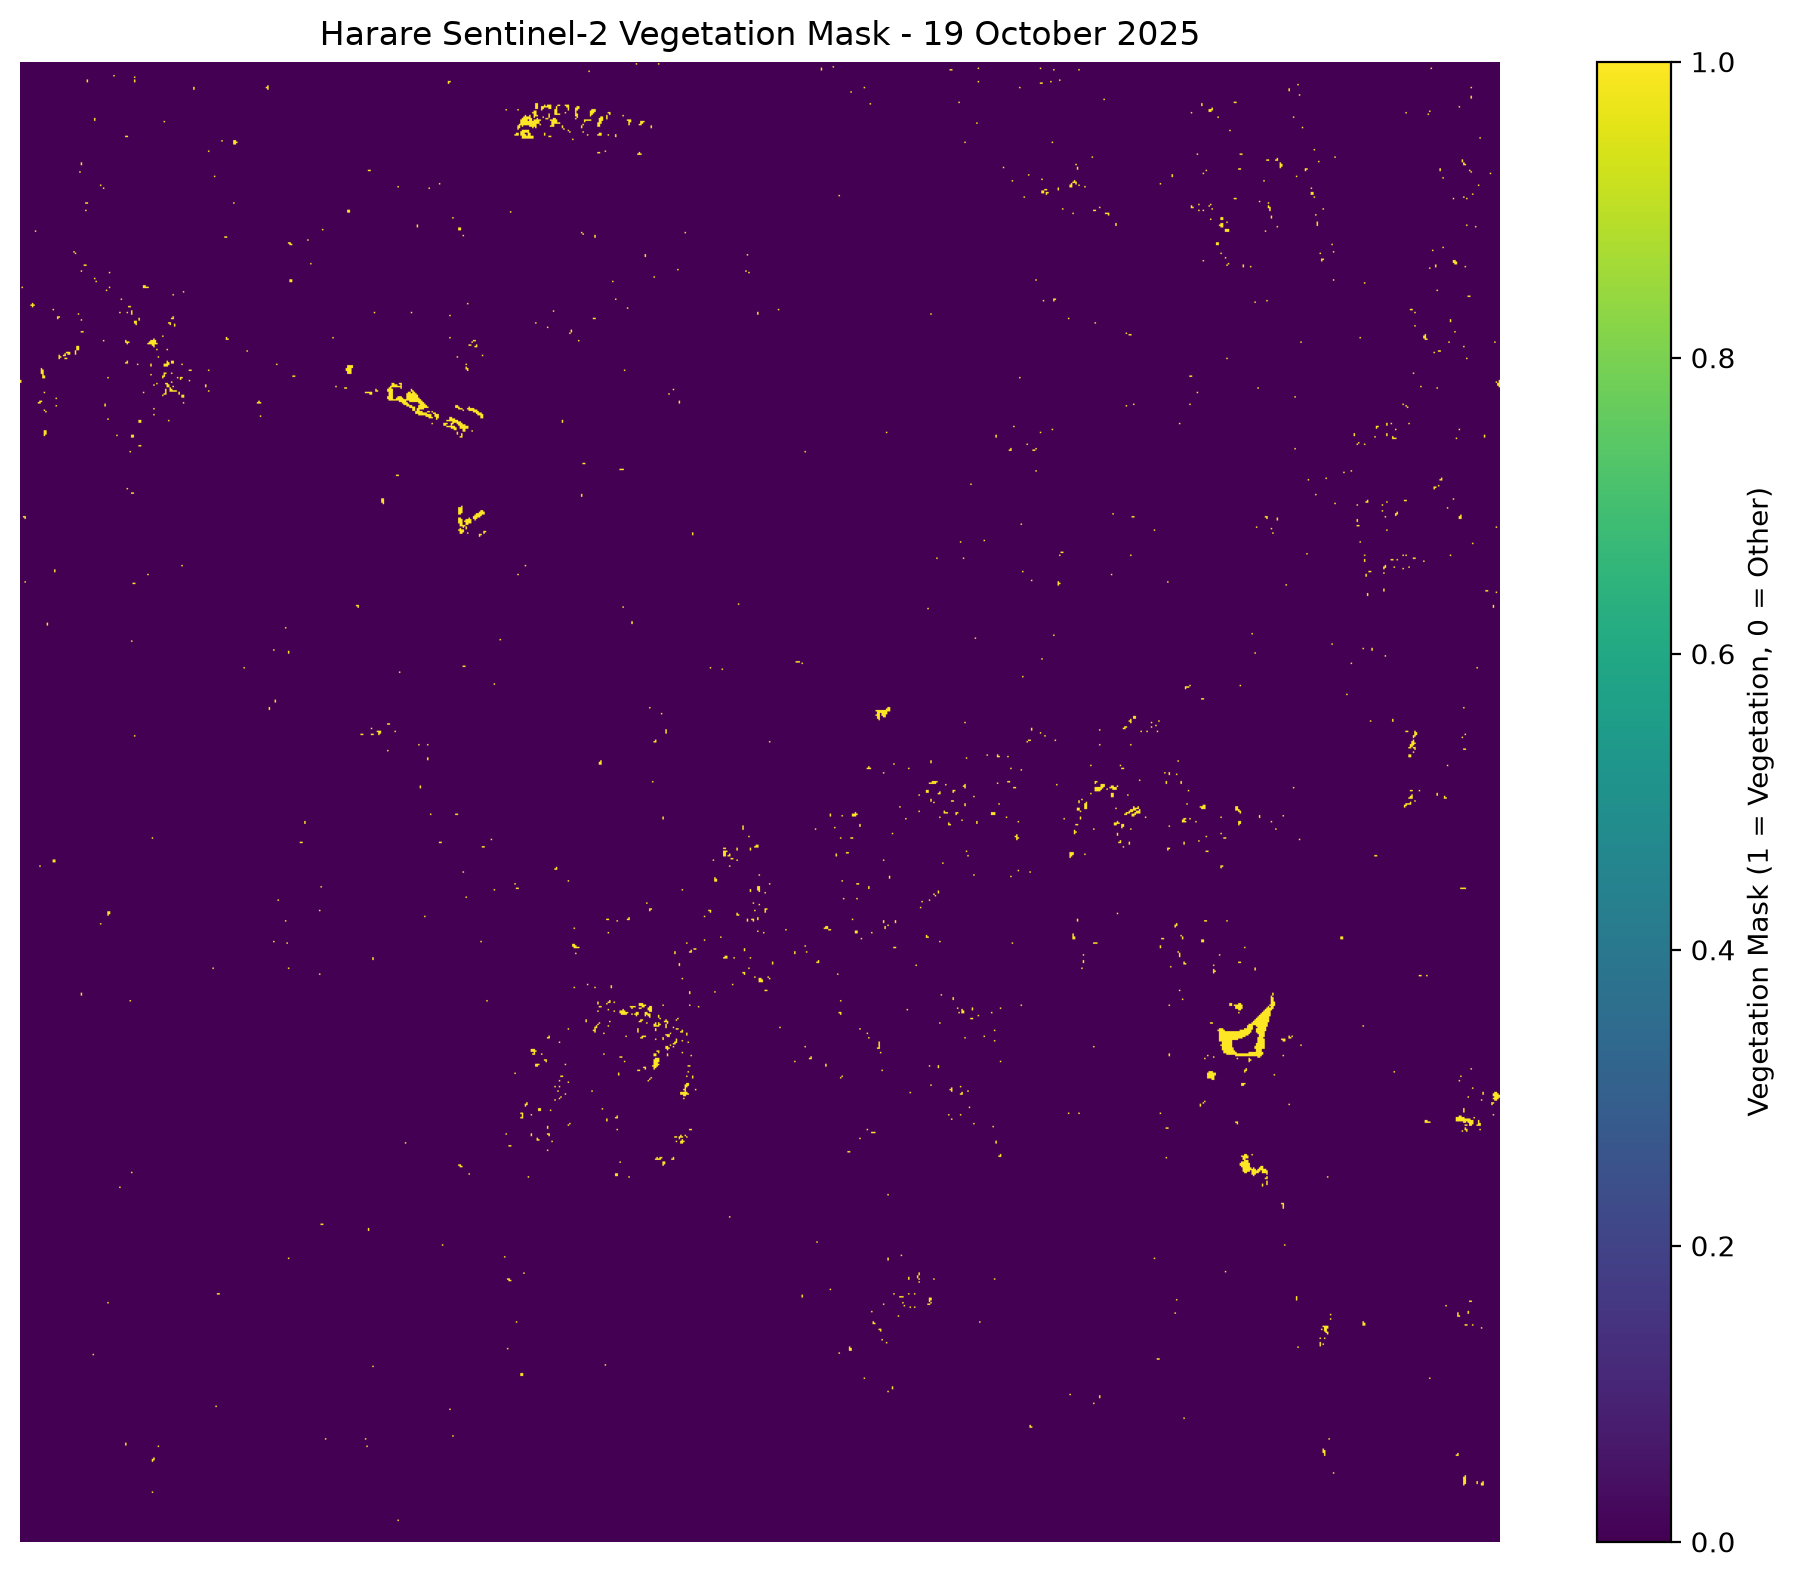
\includegraphics[width=0.82\textwidth]{harare_vegetation_mask_20251019.png}
		\caption{Exploratory vegetation mask derived from the Sentinel-2
			image for 19 October 2025.}
		\label{fig:harare-vegetation-mask}
	\end{figure}
	
	The vegetation mask provides a threshold-based view of pixels selected
	by the vegetation-masking procedure. It should be interpreted together
	with the NDVI map, since the chosen threshold and the surface conditions
	can affect which pixels are included. The mask alone does not establish
	land-cover type or confirm the presence of actively photosynthesizing
	vegetation at every selected pixel.
	
	\begin{figure}[H]
		\centering
		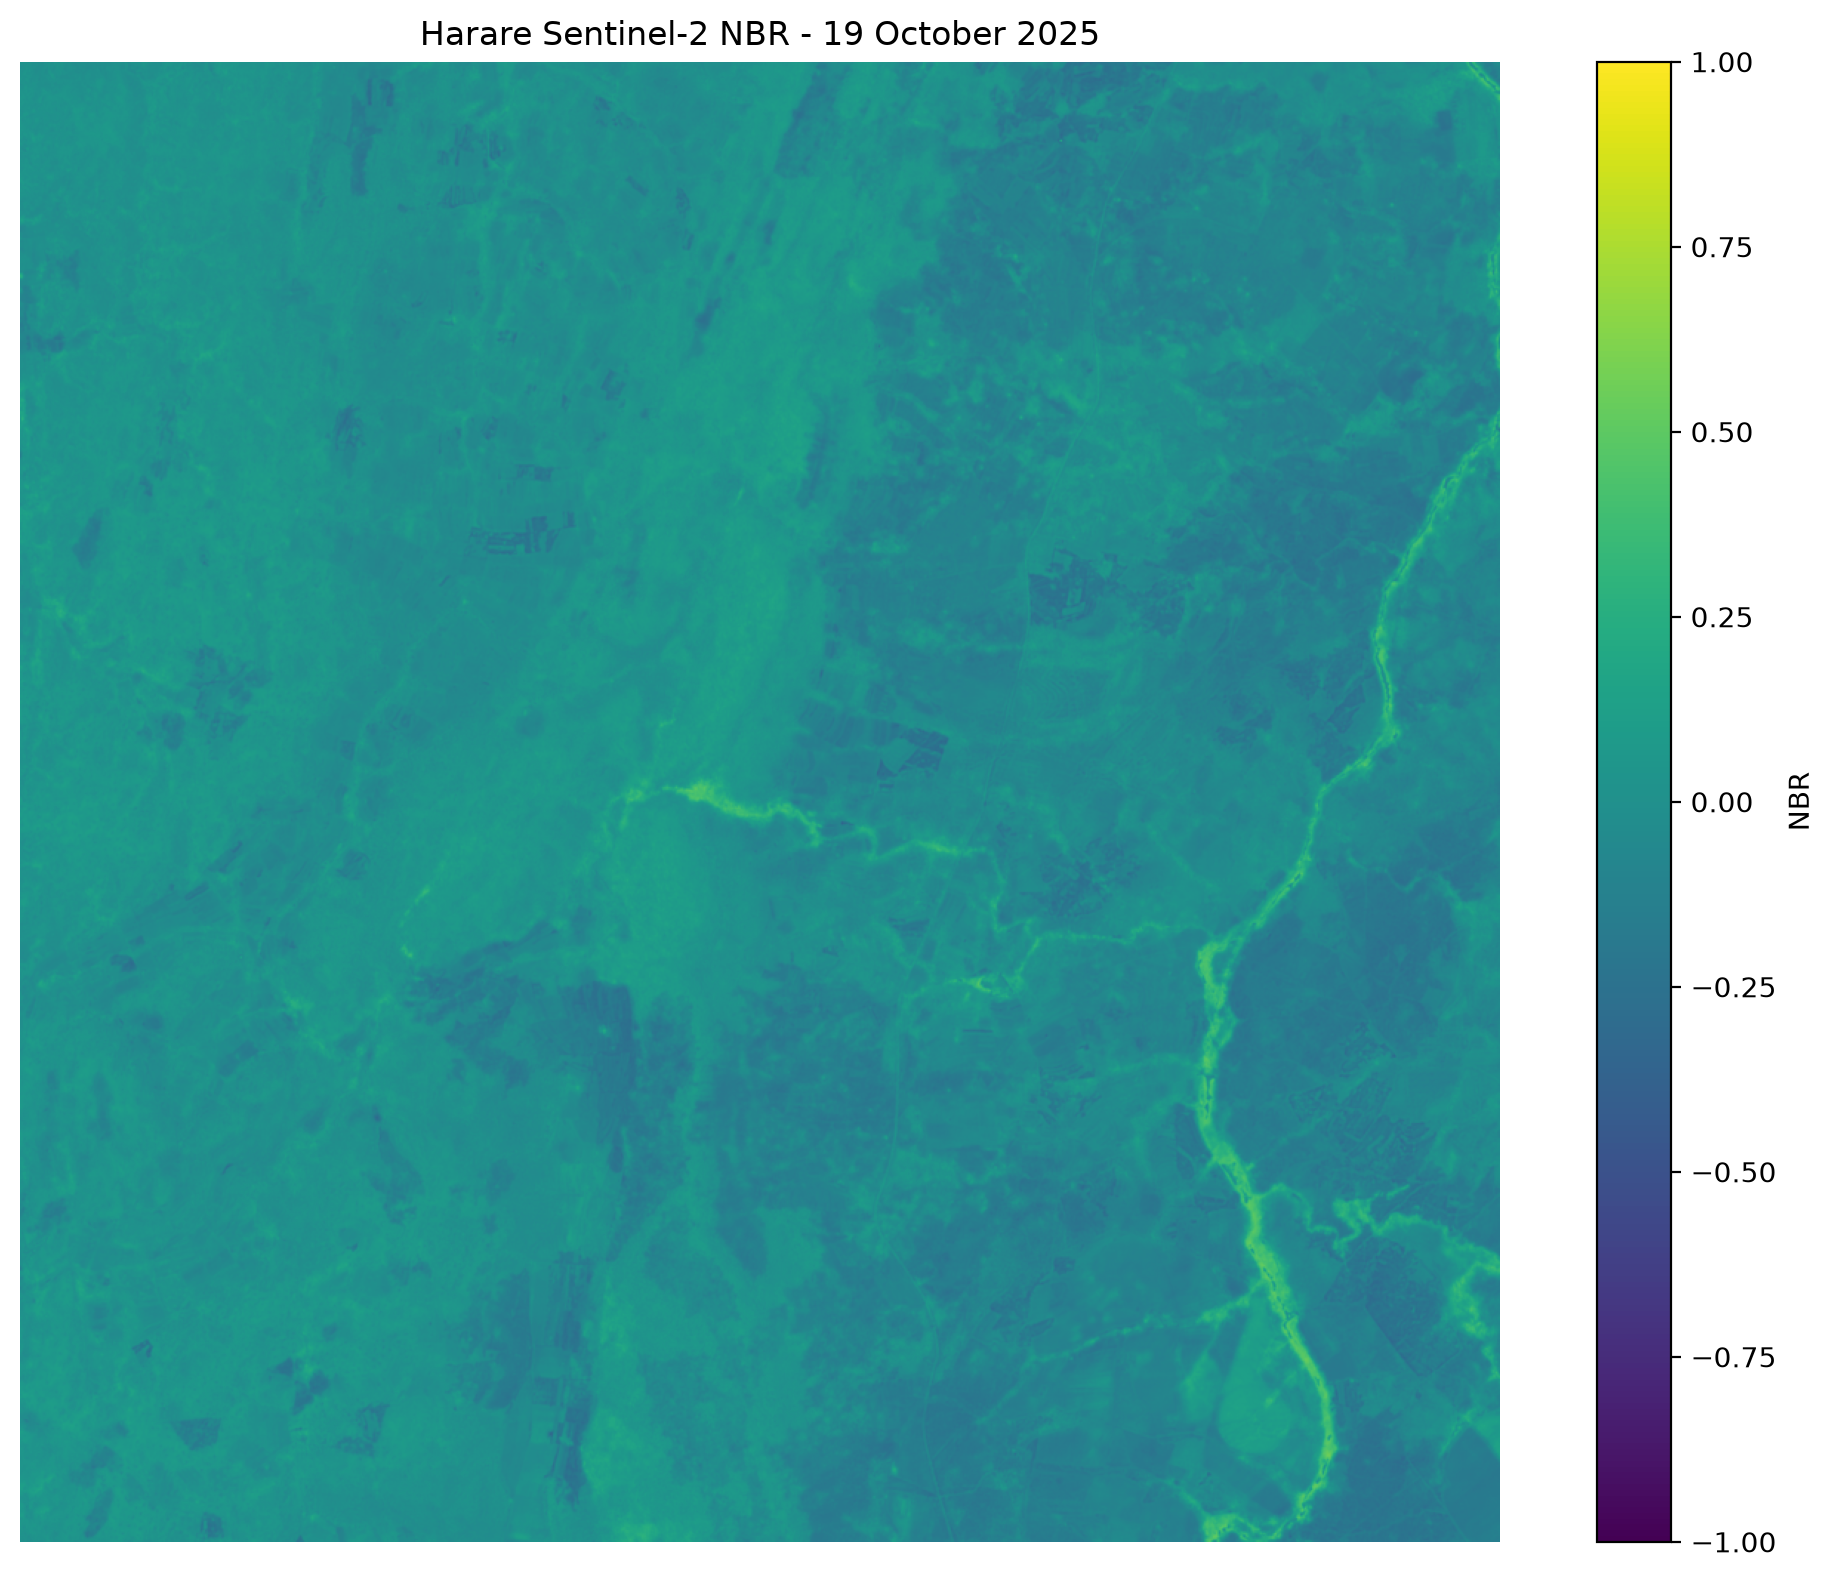
\includegraphics[width=0.82\textwidth]{harare_nbr_map_20251019.png}
		\caption{NBR map derived from the Sentinel-2 image for
			19 October 2025.}
		\label{fig:harare-nbr}
	\end{figure}
	
	The NBR raster contained 1,000,000 pixels, with a minimum of
	$-0.3684$, maximum of $0.5587$, mean of $-0.0306$, and median of
	$-0.0212$. A total of 596,698 pixels had NBR below zero. NBR values
	are influenced by land cover, vegetation and surface moisture,
	shadows, and other surface conditions. The count of negative NBR
	pixels is therefore not an estimate of burned area.
	
	\subsubsection{Bi-temporal Surface-Change Analysis}
	
	\begin{figure}[H]
		\centering
		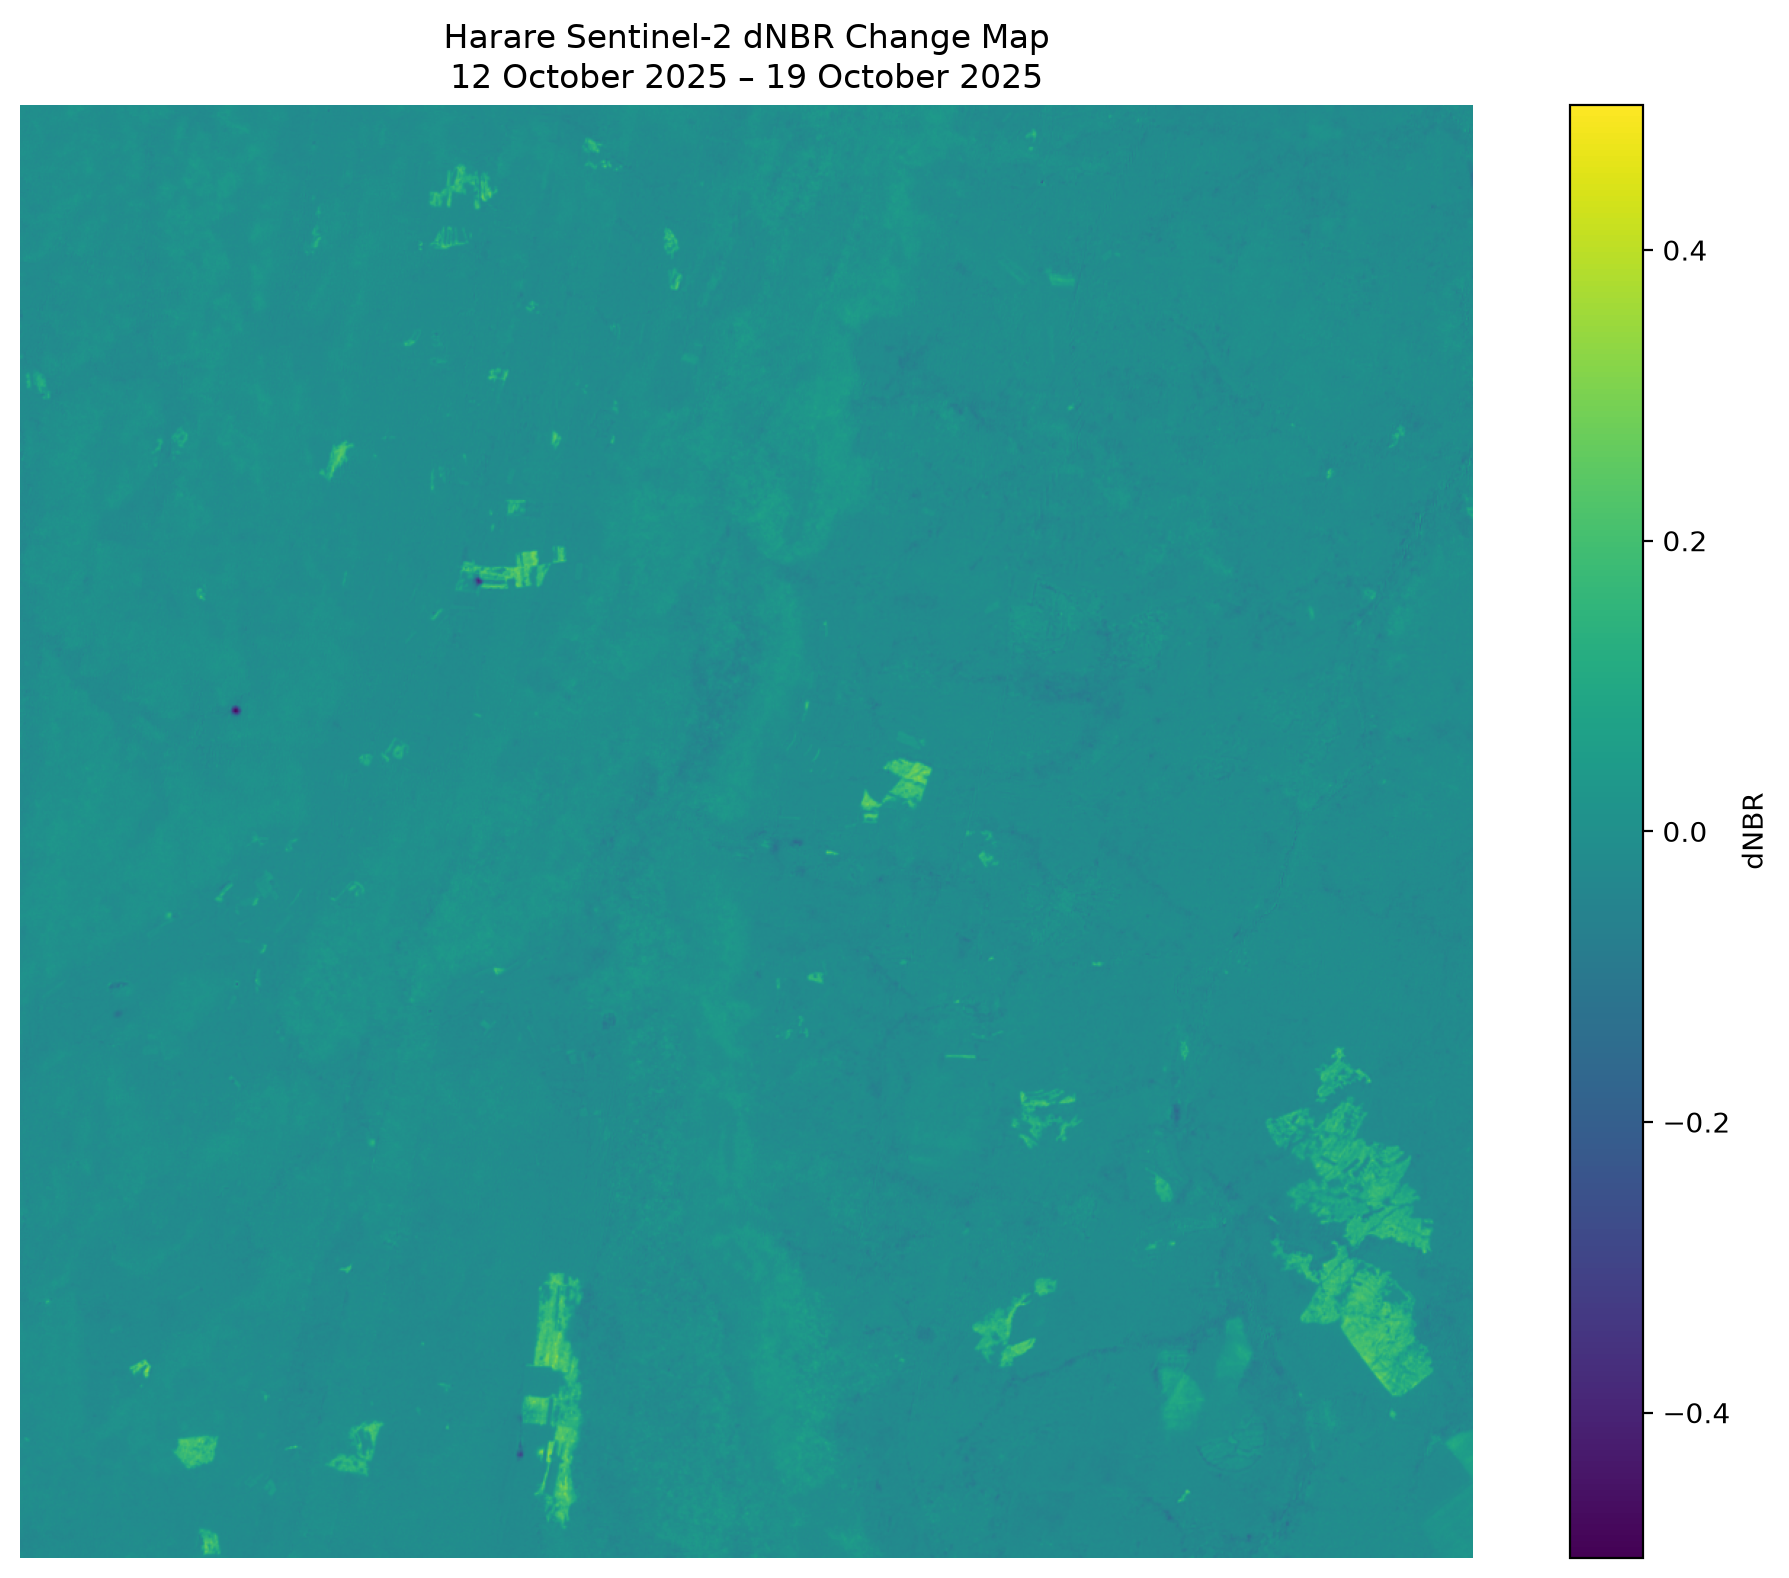
\includegraphics[width=0.82\textwidth]{harare_dnbr_map_20251012_20251019.png}
		\caption{Continuous dNBR map comparing 12 October and
			19 October 2025. Positive values indicate a reduction in NBR
			under the sign convention used in this study.}
		\label{fig:harare-dnbr-continuous}
	\end{figure}
	
	The dNBR raster had a minimum of $-0.4731$, maximum of $0.3367$,
	and mean of $-0.0091$. Most pixels were close to the little-or-no-change
	range, while smaller areas showed positive or negative differences.
	Positive dNBR values indicate a reduction in NBR under the sign
	convention used here and may flag candidate surface change. However,
	differences between the two dates can also arise from changes in
	vegetation or moisture, agricultural activity, illumination, residual
	cloud or shadow effects, or image-registration errors. The map is
	therefore treated as a candidate surface-change indicator, not evidence
	of a confirmed fire.
	
	\begin{figure}[H]
		\centering
		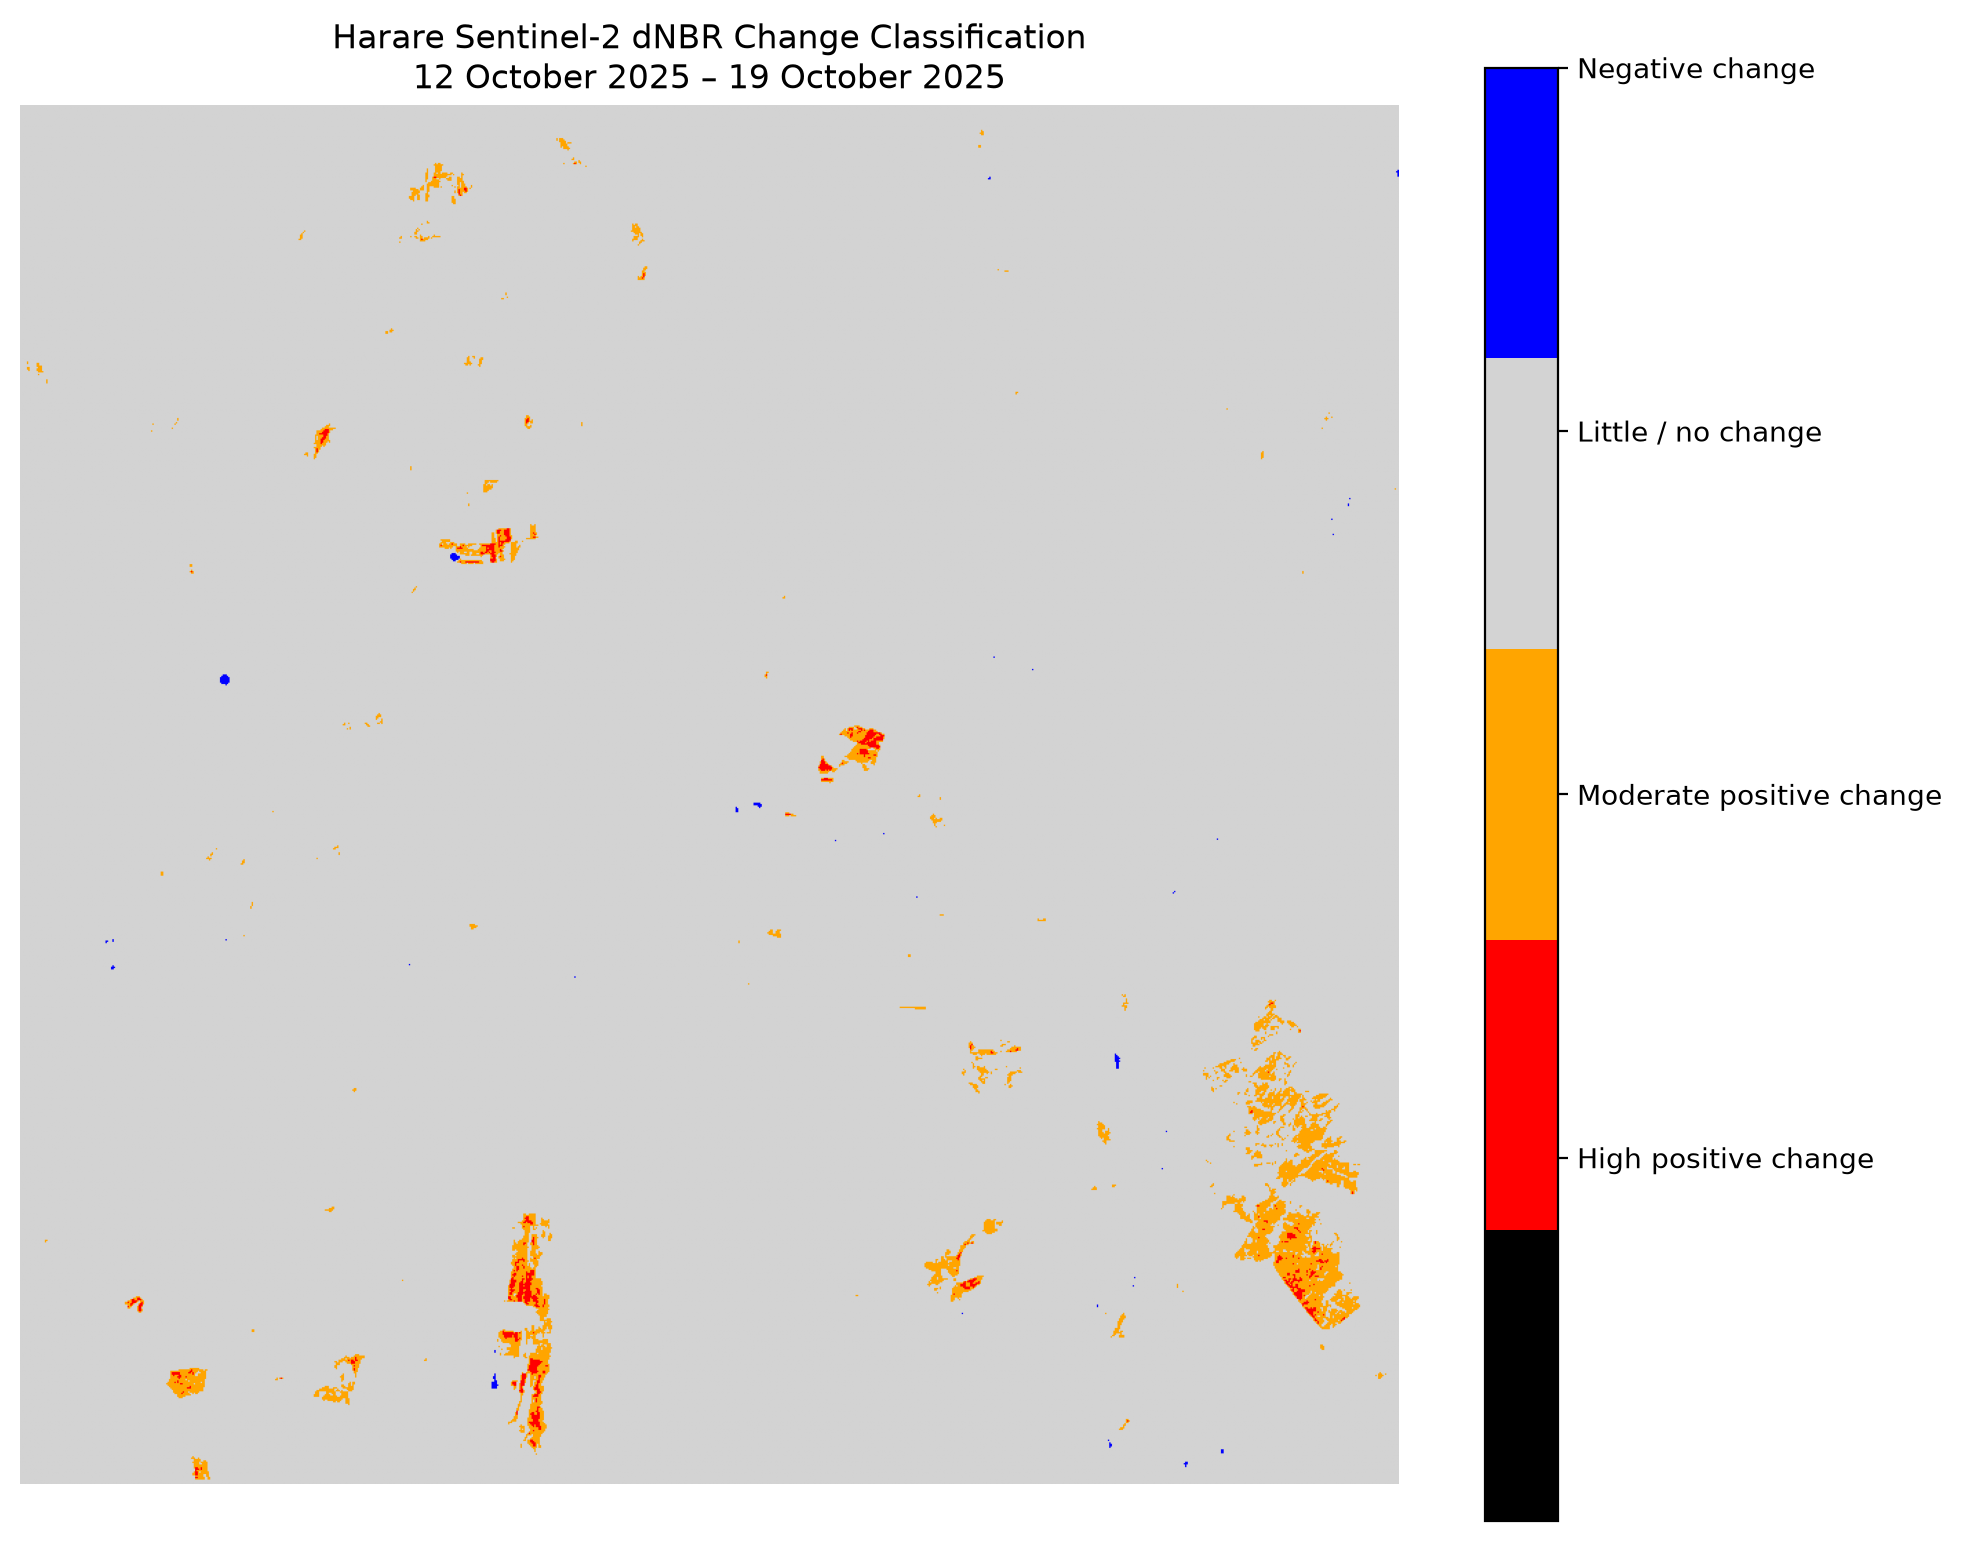
\includegraphics[width=0.82\textwidth]{harare_dnbr_classified_map_20251012_20251019.png}
		\caption{Exploratory four-class dNBR map for the 12--19 October
			2025 comparison.}
		\label{fig:harare-dnbr-classes}
	\end{figure}
	
	Table~\ref{tab:dnbr-classes} summarises the classified pixel counts.
	The area values are provisional calculations assuming that every valid
	pixel represents a $10\,\mathrm{m}\times10\,\mathrm{m}$ ground cell.
	They should not be treated as verified geographic areas until the
	raster coordinate reference system (CRS), geotransform, and spatial
	alignment have been checked.
	
	\begin{table}[H]
		\centering
		\caption{Exploratory dNBR class distribution for Harare}
		\label{tab:dnbr-classes}
		\small
		\begin{tabular}{p{4.4cm}rrr}
			\toprule
			\textbf{Class} & \textbf{Pixels} & \textbf{Share} &
			\textbf{Provisional area (km$^2$)}\\
			\midrule
			High positive change ($\mathrm{dNBR}\geq0.20$) & 1,540 & 0.15\% & 0.1540\\
			Moderate positive change ($0.10\leq\mathrm{dNBR}<0.20$) & 12,102 & 1.21\% & 1.2102\\
			Little or no change ($-0.10\leq\mathrm{dNBR}<0.10$) & 986,143 & 98.61\% & 98.6143\\
			Negative change ($\mathrm{dNBR}<-0.10$) & 215 & 0.02\% & 0.0215\\
			\midrule
			Combined positive classes & 13,642 & 1.36\% & 1.3642\\
			\bottomrule
		\end{tabular}
	\end{table}
	
	The two positive classes contained 13,642 pixels, equivalent to
	$1.3642\,\mathrm{km}^2$ under the nominal pixel-size assumption.
	This is the area assigned to the positive dNBR classes, not a measured
	burned area. The classified output depends on the selected thresholds
	and the quality and alignment of the input rasters.
	
	\begin{figure}[H]
		\centering
		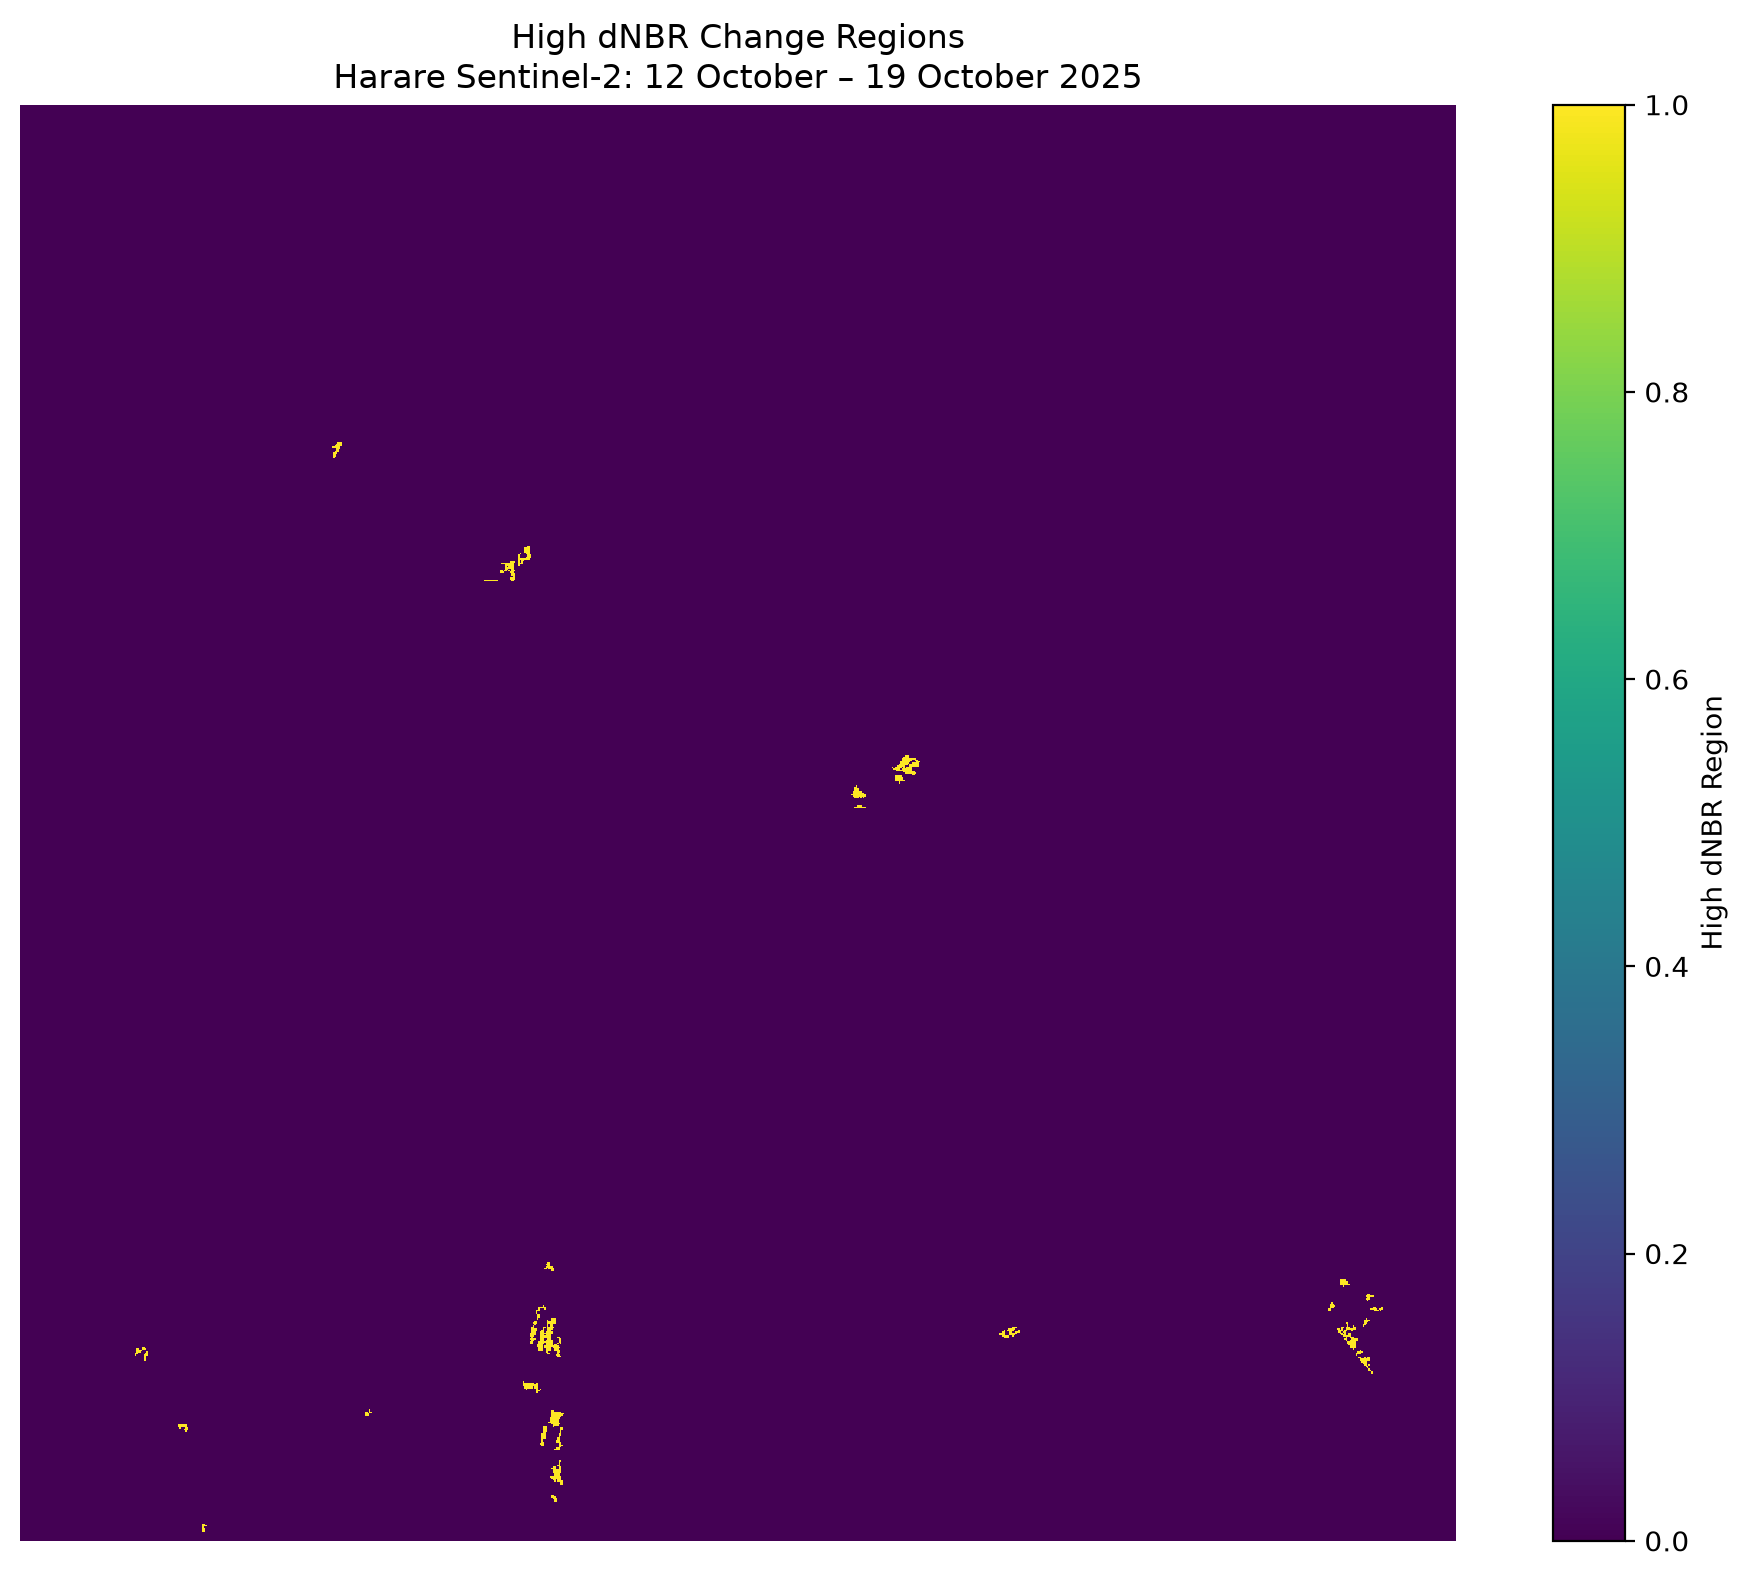
\includegraphics[width=0.82\textwidth]{harare_high_dnbr_regions_map_20251012_20251019.png}
		\caption{Connected candidate high-dNBR regions after applying the
			exploratory threshold and minimum-region-size filter.}
		\label{fig:harare-high-dnbr-regions}
	\end{figure}
	
	The connected-region procedure initially identified 1,540 pixels
	across 150 candidate regions at the high-positive threshold. After
	excluding regions smaller than 10 pixels, 32 regions containing
	1,264 pixels remained; 276 pixels belonging to smaller regions were
	excluded. The largest retained region contained 197 pixels. Under the
	nominal 10 m pixel assumption, this corresponds to $0.0197\,\mathrm{km}^2$
	or 1.97 hectares. These are provisional raster-based summaries, not
	confirmed disturbance or fire extents.
	
	\subsubsection{Spatial Quality Control and Methodological Caveats}
	
	A spatial metadata discrepancy was identified during quality control:
	the tie point reported for a separate disturbance-region raster differs
	from that of the dNBR and classified dNBR rasters. Before pixel-wise
	comparison, centroid interpretation, or final area reporting, all
	rasters should be checked and, where necessary, reprojected or aligned
	to a common verified coordinate reference system and grid. In addition,	agricultural harvesting, soil disturbance, moisture changes, and cloud or
	shadow differences can produce dNBR patterns that resemble burning.
	Independent validation using suitable high-resolution imagery or field
	information is needed to establish the cause of any mapped change.
	
	\FloatBarrier
	
	\subsection{Interpretation of Model Performance}
	
	The XGBoost results indicate that predictions were close to the
	observed test temperatures on average. RMSE is greater than MAE,
	which is consistent with RMSE assigning more weight to larger
	prediction errors. The high reported $R^2$ indicates that the model
	accounted for a large proportion of the variation in the evaluated
	test targets, although goodness-of-fit measures should be interpreted
	with error metrics and the test design \cite{gneiting2011,jolliffe2012}.
	
	Aggregate metrics can hide differences among cities, seasons, and
	weather conditions. Further evaluation should report per-city
	errors, seasonal performance, and error distributions. Comparisons
	against additional baselines and suitable external forecasts could
	also provide a more complete assessment of practical value.
	
	% --------------------------------------------------
	% 5. SYSTEM IMPLEMENTATION
	% --------------------------------------------------
	\section{System Implementation}
	
	\subsection{System Architecture}
	
	The selected XGBoost model was integrated into an application
	consisting of a Streamlit frontend, a FastAPI backend, and the
	trained model artifact. The frontend sends prediction requests to
	the backend, which validates the request, prepares the model inputs,
	obtains a prediction, and returns the result to the dashboard.
	
	\begin{center}
		\texttt{User}
		$\rightarrow$ \texttt{Streamlit}
		$\rightarrow$ \texttt{FastAPI}
		$\rightarrow$ \texttt{XGBoost}
		$\rightarrow$ \texttt{FastAPI}
		$\rightarrow$ \texttt{Streamlit}
	\end{center}
	
	\subsection{FastAPI Backend}
	
	FastAPI exposes prediction functionality through HTTP endpoints.
	The service provides endpoints for basic API information, health
	checking, supported cities, and predictions. Interactive API
	documentation is available through Swagger UI.
	
	\begin{table}[H]
		\centering
		\caption{Principal API endpoints}
		\label{tab:api-endpoints}
		\begin{tabular}{lp{9cm}}
			\toprule
			\textbf{Endpoint} & \textbf{Purpose}\\
			\midrule
			\texttt{/} & Returns basic API information.\\
			\texttt{/health} & Reports health status and model information.\\
			\texttt{/cities} & Returns supported city options.\\
			\texttt{/predict} & Accepts prediction inputs and returns a prediction.\\
			\texttt{/docs} & Provides interactive API documentation.\\
			\bottomrule
		\end{tabular}
	\end{table}
	
	The deployed backend is hosted on Render at:
	\url{https://zimbabwe-weather-intelligence-macroedtech.onrender.com/}
	
	\subsection{Streamlit Dashboard}
	
	Streamlit provides an interface for selecting a supported city,
	providing the prediction date and time, entering weather variables,
	and viewing the model output. The dashboard is hosted on Streamlit
	Community Cloud at:
	\url{https://zimbabwe-weather-intelligence-macroedtech-nv4fr3n3byeb8vtgxfza.streamlit.app/}
	
	The frontend communicates with the backend using the
	\texttt{API\_BASE\_URL} environment variable. This allows the
	dashboard and API to be deployed independently.
	
	\subsection{Prediction Workflow}
	
	The user selects a city and supplies the required weather values.
	The dashboard sends these values to the prediction endpoint. The
	backend validates the request and passes the prepared features to
	the trained XGBoost model. The resulting prediction is returned
	through the API and displayed in the dashboard.
	
	The application supports user-supplied inputs and what-if analysis.
	It does not independently obtain current weather observations.
	The validity of an individual prediction therefore depends partly
	on the quality, relevance, and timing of the supplied inputs.
	
	\subsection{Deployment}
	
	The FastAPI backend was deployed on Render and the Streamlit
	dashboard on Streamlit Community Cloud. The dashboard's API base
	URL was configured through the deployment environment's settings.
	The deployed API health endpoint returned a healthy status and
	identified XGBoost as the model used for one-hour-ahead temperature
	prediction. The public dashboard was tested with the four supported
	cities. These checks demonstrate successful operation for the
	tested workflows, rather than guaranteeing uninterrupted service.
	
	\subsection{Separate Satellite Processing Workflow}
	
	The exploratory satellite workflow was implemented separately from
	the deployed weather prediction service. It used Sentinel-2 imagery
	to generate a true-colour view, NDVI and NBR rasters, a two-date dNBR
	raster, classified change pixels, and connected candidate high-change
	regions. The resulting maps and summary tables were saved as analysis
	outputs for inspection. They are not requested by the FastAPI
	prediction endpoint, are not displayed as XGBoost temperature
	predictions, and were not used to train or evaluate the deployed
	weather model.
	
	The satellite workflow remains experimental. Before the maps are used
	for operational environmental monitoring, the processing should
	verify scene identity and cloud/shadow masking, CRS and geotransform,
	spatial alignment between dates and derived products, threshold
	sensitivity, and the relationship between detected changes and
	independent reference information.
	
	% --------------------------------------------------
	% 6. TESTING
	% --------------------------------------------------
	\section{Testing and Verification}
	
	\subsection{Automated API Testing}
	
	An automated test suite in \texttt{tests/test\_api.py} was run in
	the development environment. Seven tests passed. The tests covered:
	\begin{enumerate}[leftmargin=*]
		\item The root endpoint response.
		\item The health endpoint.
		\item The supported cities endpoint.
		\item A valid prediction request.
		\item Rejection of an unknown city.
		\item Rejection of an invalid date-time value.
		\item Rejection of a request with a missing required field.
	\end{enumerate}
	
	The result of seven passing tests confirms the tested behaviours
	in the development environment. It does not imply that every
	possible input, deployment failure, or production condition has
	been tested.
	
	\subsection{Deployment Verification}
	
	Deployment checks included opening the public API health endpoint,
	accessing Swagger documentation, and using the dashboard to
	generate predictions for the four supported cities. These checks
	provided evidence that the frontend and backend were accessible
	and that the tested prediction workflow operated.
	
	\subsection{Testing Limitations}
	
	Further testing could include:
	\begin{itemize}[leftmargin=*]
		\item Integration tests covering the complete dashboard-to-API flow.
		\item Boundary tests for numerical weather inputs.
		\item Handling of API timeouts and unavailable backend services.
		\item Tests for malformed and extreme inputs.
		\item Regression tests after model or feature changes.
		\item Performance testing under concurrent requests.
	\end{itemize}
	
	% --------------------------------------------------
	% 7. DISCUSSION
	% --------------------------------------------------
	\section{Discussion}
	
	XGBoost achieved the strongest reported test performance among
	the six evaluated approaches. Its results were slightly better
	than those of Random Forest and substantially better than the
	persistence baseline. Tree-based ensemble methods can represent
	nonlinear relationships and interactions among structured weather
	features; this is a plausible interpretation of their performance,
	but the results alone do not prove why the difference occurred.
	
	Feature importance indicates that current temperature and the
	24-hour temperature lag were particularly influential under the
	importance measure used. This is consistent with the value of
	recent observations and daily temporal patterns for short-horizon
	temperature prediction. Feature importance is model-specific and
	should not be interpreted causally.
	
	The LSTM experiments did not outperform the tree-based models in
	the reported comparison. This illustrates that a more complex
	sequence architecture does not automatically produce better
	predictions. Results can depend on sequence preparation, model
	configuration, training procedures, and how the available
	information is represented.
	
	An important engineering outcome is the integration of the trained
	model into a deployed application. A model becomes more accessible
	when it can be queried through a documented API and an interactive
	dashboard. Separate deployment of the frontend and backend also
	provides a modular foundation for subsequent development.
	
	The practical significance of the metrics nevertheless requires
	careful interpretation. The evaluation uses a particular historical
	test period and four selected cities. Additional analysis is needed
	to determine how performance varies by location, season, and
	unusual weather conditions. The system should be understood as a
	historical-data-based, one-hour-ahead temperature prediction
	prototype, not as a replacement for official meteorological
	forecasting services.
	
	% --------------------------------------------------
	% 8. LIMITATIONS AND FUTURE WORK
	% --------------------------------------------------
	\section{Limitations and Future Work}
	
	\subsection{Limitations}
	
	\textbf{Geographical coverage:} The study covers four cities and
	does not establish generalisation to all of Zimbabwe.
	
	\textbf{Prediction target:} The deployed model predicts temperature
	one hour ahead. The results cannot be assumed to apply to rainfall
	prediction, long-range forecasting, or other meteorological targets.
	
	\textbf{Input dependence:} The application uses supplied weather
	values and does not independently retrieve current observations.
	Prediction quality therefore depends partly on the inputs provided.
	
	\textbf{Evaluation scope:} Reported performance is based on the 2025
	test period. Further testing is required to assess performance during
	extreme weather, across individual cities, and over additional
	future periods.
	
	\textbf{Model comparison:} The metrics do not establish that every
	model was optimally tuned or that all possible forecasting
	approaches were considered.
	
	\textbf{Operational reliability:} Free-tier hosting services may
	experience cold starts, temporary delays, or service limitations.
	Operational use would require additional monitoring and reliability
	testing.
	
	\subsection{Future Work}
	
	Future development should prioritise:
	\begin{enumerate}[leftmargin=*]
		\item \textbf{Expanded evaluation:} Report city-specific and
		seasonal performance, examine error distributions, and evaluate
		model behaviour during extreme weather.
		\item \textbf{Improved forecasting inputs:} Investigate reliable
		ways to obtain current observations or forecast inputs while
		maintaining clear data provenance.
		\item \textbf{Uncertainty estimation:} Explore methods for
		communicating prediction uncertainty rather than presenting a
		point estimate alone.
		\item \textbf{Application monitoring:} Introduce structured
		logging, availability checks, integration tests, and monitoring
		of failed prediction requests.
		\item \textbf{Satellite and environmental analysis:} Validate the
		exploratory Sentinel-2 NDVI, NBR, and dNBR products by checking
		coordinate reference systems, geotransforms, scene registration,
		cloud and shadow masking, threshold sensitivity, and independent
		reference data. The current positive dNBR pixels are candidate
		surface changes and must not be reported as confirmed burned area.
		The satellite experiment remains separate from the deployed
		XGBoost temperature-prediction pipeline.
		\item \textbf{Weather intelligence assistant:} Investigate
		retrieval-augmented generation and open-weight language models
		to provide evidence-based explanations. Such a component should
		distinguish retrieved evidence from model predictions.
		\item \textbf{Reproducibility:} Document data retrieval
		parameters, feature definitions, model configurations, software
		versions, and procedures required to reproduce the experiments.
	\end{enumerate}
	
	% --------------------------------------------------
	% 9. CONCLUSION
	% --------------------------------------------------
	\section{Conclusion}
	
	This study presented Zimbabwe Weather Intelligence, an end-to-end
	machine learning application for one-hour-ahead temperature
	prediction across Harare, Bulawayo, Mutare, and Gweru. The project
	used 385,728 hourly weather records covering 2015--2025 and compared
	a persistence baseline, Linear Regression, Random Forest, XGBoost,
	and two LSTM configurations.
	
	Using the reported 2025 test metrics, XGBoost achieved the best
	overall performance among the evaluated models, with an MAE of
	0.3448$^\circ$C, an RMSE of 0.5210$^\circ$C, and an $R^2$ of 0.9882.
	The feature-importance output identified current temperature and
	the 24-hour temperature lag as the two most influential features
	under the reported measure.
	
	The selected model was integrated into a FastAPI backend and a
	Streamlit dashboard. The application was deployed online, its API
	health endpoint and documentation were checked, and seven core API
	tests passed in the development environment.
	
	The findings demonstrate the feasibility of building a practical
	temperature prediction application using historical data,
	machine learning, and web technologies. Further work is needed to
	evaluate performance across cities, seasons, and extreme conditions;
	improve operational monitoring; estimate prediction uncertainty;
	and document the experiments for reproducibility. A separate
	exploratory Sentinel-2 analysis generated NDVI, NBR, and dNBR maps
	for a Harare-area comparison between 12 and 19 October 2025. The
	positive dNBR classes identified candidate surface changes only;
	their geographic alignment and interpretation require further
	validation, and they do not establish a confirmed fire event or
	burned area. This satellite experiment was not part of the deployed
	XGBoost model evaluated in this study.
	
	% --------------------------------------------------
	% REFERENCES
	% --------------------------------------------------
	\begin{thebibliography}{15}
		
		\bibitem{breiman2001}
		Breiman, L. (2001). Random forests. \textit{Machine Learning, 45}, 5--32.
		\url{https://doi.org/10.1023/A:1010933404324}
		
		\bibitem{chen2016}
		Chen, T., \& Guestrin, C. (2016). XGBoost: A scalable tree boosting system.
		In \textit{Proceedings of the 22nd ACM SIGKDD International Conference on
			Knowledge Discovery and Data Mining} (pp. 785--794).
		\url{https://doi.org/10.1145/2939672.2939785}
		
		\bibitem{hochreiter1997}
		Hochreiter, S., \& Schmidhuber, J. (1997). Long short-term memory.
		\textit{Neural Computation, 9}(8), 1735--1780.
		\url{https://doi.org/10.1162/neco.1997.9.8.1735}
		
		\bibitem{hyndman2021}
		Hyndman, R. J., \& Athanasopoulos, G. (2021).
		\textit{Forecasting: Principles and Practice} (3rd ed.). OTexts.
		\url{https://otexts.com/fpp3/}
		
		\bibitem{openmeteo}
		Open-Meteo. (n.d.). \textit{Historical Weather API}.
		\url{https://open-meteo.com/en/docs/historical-weather-api}
		
		\bibitem{copernicusdataspace}
		Copernicus Data Space Ecosystem. (n.d.).
		\textit{Sentinel-2 mission and Earth observation data access}.
		\url{https://dataspace.copernicus.eu/}
		
		\bibitem{xgboostdocs}
		XGBoost Developers. (n.d.). \textit{XGBoost Documentation}.
		\url{https://xgboost.readthedocs.io/}
		
		\bibitem{bergmeir2018}
		Bergmeir, C., Hyndman, R. J., \& Koo, B. (2018). A note on the validity
		of cross-validation for evaluating autoregressive time series prediction.
		\textit{Computational Statistics \& Data Analysis, 120}, 70--83.
		\url{https://doi.org/10.1016/j.csda.2017.11.003}
		
		\bibitem{wilks2019}
		Wilks, D. S. (2019). \textit{Statistical Methods in the Atmospheric Sciences}
		(4th ed.). Elsevier.
		\url{https://doi.org/10.1016/C2017-0-03921-6}
		
		\bibitem{scikitlearnmetrics}
		Scikit-learn developers. (n.d.). \textit{Metrics and scoring: Quantifying the quality of predictions}.
		\url{https://scikit-learn.org/stable/modules/model_evaluation.html}
		
		\bibitem{drusch2012}
		Drusch, M., Del Bello, U., Carlier, S., Colin, O., Fernandez, V.,
		Gascon, F., Hoersch, B., Isola, C., Laberinti, P., Martimort, P.,
		Meygret, A., Spoto, F., Sy, O., Marchese, F., \& Bargellini, P. (2012).
		Sentinel-2: ESA's optical high-resolution mission for GMES operational services.
		\textit{Remote Sensing of Environment, 120}, 25--36.
		\url{https://doi.org/10.1016/j.rse.2011.11.026}
		
		\bibitem{tucker1979}
		Tucker, C. J. (1979). Red and photographic infrared linear combinations
		for monitoring vegetation. \textit{Remote Sensing of Environment, 8}(2), 127--150.
		\url{https://doi.org/10.1016/0034-4257(79)90013-0}
		
		\bibitem{keybenson2006}
		Key, C. H., \& Benson, N. C. (2006). Landscape assessment: Ground measure
		of severity, the Composite Burn Index; and remote sensing of severity,
		the Normalized Burn Ratio. In D. C. Lutes et al. (Eds.),
		\textit{FIREMON: Fire effects monitoring and inventory system}.
		USDA Forest Service, Rocky Mountain Research Station, General Technical
		Report RMRS-GTR-164-CD.
		\url{https://www.fs.usda.gov/rm/pubs/rmrs_gtr164/rmrs_gtr164_13_land_assess.pdf}
		
		\bibitem{gneiting2011}
		Gneiting, T. (2011). Making and evaluating point forecasts.
		\textit{Journal of the American Statistical Association, 106}(494), 746--762.
		\url{https://doi.org/10.1198/jasa.2011.r10138}
		
		\bibitem{jolliffe2012}
		Jolliffe, I. T., \& Stephenson, D. B. (Eds.). (2012).
		\textit{Forecast Verification: A Practitioner's Guide in Atmospheric Science}
		(2nd ed.). Wiley.
		\url{https://doi.org/10.1002/9781119960003}
		
	\end{thebibliography}
	
\end{document}
